\documentclass[11pt]{article}
\usepackage[preprint]{acl}
\usepackage{times}
\usepackage{latexsym}
\usepackage[T1]{fontenc}
\usepackage[utf8]{inputenc}
\usepackage{microtype,booktabs,graphicx,amsmath,amssymb,xcolor}
\usepackage{placeins,enumitem,array}
\graphicspath{{figures/}}
\setcounter{dbltopnumber}{3}
\renewcommand{\dbltopfraction}{0.85}
\renewcommand{\dblfloatpagefraction}{0.7}
\newcommand{\PBpaired}{100}
\newcommand{\PBpassLLM}{41.0}
\newcommand{\PBcpLLM}{81.3}
\newcommand{\PBdiffLLM}{--}
\newcommand{\PBpLLM}{=--}
\newcommand{\PBtokLLM}{29k}
\newcommand{\PBpassSel}{37.0}
\newcommand{\PBcpSel}{80.2}
\newcommand{\PBdiffSel}{$-$4.0 [$-$13.0, +5.0]}
\newcommand{\PBpSel}{=0.52}
\newcommand{\PBtokSel}{119k}
\newcommand{\PBpassTool}{7.0}
\newcommand{\PBcpTool}{44.3}
\newcommand{\PBdiffTool}{$-$34.0 [$-$45.0, $-$23.0]}
\newcommand{\PBpTool}{<0.001}
\newcommand{\PBtokTool}{18k}
\newcommand{\PBpassRep}{--}
\newcommand{\PBcpRep}{--}
\newcommand{\PBdiffRep}{--}
\newcommand{\PBpRep}{=--}
\newcommand{\PBtokRep}{--}
\newcommand{\PBnfTasks}{7}
\newcommand{\PBnfDiff}{$-$14.3 [$-$57.1, +28.6]}
\newcommand{\PBnfDisc}{3}
\newcommand{\PRSelLLMn}{100}
\newcommand{\PRSelLLMdiff}{$-$4.0 [$-$13.0, +5.0]}
\newcommand{\PRSelLLMcp}{$-$1.1 [$-$4.8, +2.7]}
\newcommand{\PRSelLLMp}{=0.52}
\newcommand{\PRSelLLMx}{37.0}
\newcommand{\PRSelLLMy}{41.0}
\newcommand{\PRSelLLMDR}{+1.8 [$-$4.2, +7.7]}
\newcommand{\PRSelLLMCR}{$-$1.2 [$-$5.3, +3.2]}
\newcommand{\PRSelLLMAE}{+5.1 [$-$2.4, +13.7]}
\newcommand{\PRSelLLMDO}{$-$5.1 [$-$14.1, +3.0]}
\newcommand{\PRToolCtln}{82}
\newcommand{\PRToolCtldiff}{$-$25.6 [$-$36.6, $-$14.6]}
\newcommand{\PRToolCtlcp}{$-$36.7 [$-$44.4, $-$28.9]}
\newcommand{\PRToolCtlp}{<0.001}
\newcommand{\PRToolCtlx}{7.3}
\newcommand{\PRToolCtly}{32.9}
\newcommand{\PRToolCtlDR}{$-$40.6 [$-$51.6, $-$29.3]}
\newcommand{\PRToolCtlCR}{$-$37.9 [$-$46.9, $-$28.8]}
\newcommand{\PRToolCtlAE}{$-$26.3 [$-$40.1, $-$12.8]}
\newcommand{\PRToolCtlDO}{$-$37.0 [$-$48.1, $-$25.9]}
\newcommand{\PRCtlLLMn}{82}
\newcommand{\PRCtlLLMdiff}{$-$7.3 [$-$19.5, +4.9]}
\newcommand{\PRCtlLLMcp}{+0.7 [$-$3.6, +5.3]}
\newcommand{\PRCtlLLMp}{=0.34}
\newcommand{\PRCtlLLMx}{32.9}
\newcommand{\PRCtlLLMy}{40.2}
\newcommand{\PRCtlLLMDR}{$-$0.2 [$-$6.9, +6.3]}
\newcommand{\PRCtlLLMCR}{+1.9 [$-$2.8, +7.3]}
\newcommand{\PRCtlLLMAE}{+9.5 [$-$0.6, +20.5]}
\newcommand{\PRCtlLLMDO}{$-$6.2 [$-$17.3, +4.9]}
\newcommand{\TLCallsLLM}{36.3}
\newcommand{\TLRetLLM}{31.2}
\newcommand{\TLActLLM}{3.5}
\newcommand{\TLDocLLM}{1.6}
\newcommand{\TLFirstLLM}{30.1}
\newcommand{\ENDLLM}{2}
\newcommand{\DECLLMmaxp}{--}
\newcommand{\DECLLMs}{--}
\newcommand{\DECLLMsem}{--}
\newcommand{\DECLLMfirst}{--}
\newcommand{\DECLLMdepart}{--}
\newcommand{\DECLLMerr}{--}
\newcommand{\DECLLMshort}{--}
\newcommand{\DECLLMomit}{--}
\newcommand{\TOKLLM}{29k}
\newcommand{\TLCallsSel}{31.2}
\newcommand{\TLRetSel}{26.4}
\newcommand{\TLActSel}{3.6}
\newcommand{\TLDocSel}{1.2}
\newcommand{\TLFirstSel}{24.8}
\newcommand{\ENDSel}{1}
\newcommand{\DECSelmaxp}{0.382}
\newcommand{\DECSels}{4.7}
\newcommand{\DECSelsem}{89}
\newcommand{\DECSelfirst}{21}
\newcommand{\DECSeldepart}{79}
\newcommand{\DECSelerr}{0}
\newcommand{\DECSelshort}{44}
\newcommand{\DECSelomit}{1}
\newcommand{\TOKSel}{119k}
\newcommand{\TLCallsTool}{25.7}
\newcommand{\TLRetTool}{14.2}
\newcommand{\TLActTool}{2.3}
\newcommand{\TLDocTool}{9.2}
\newcommand{\TLFirstTool}{9.9}
\newcommand{\ENDTool}{16}
\newcommand{\DECToolmaxp}{0.451}
\newcommand{\DECTools}{--}
\newcommand{\DECToolsem}{--}
\newcommand{\DECToolfirst}{--}
\newcommand{\DECTooldepart}{--}
\newcommand{\DECToolerr}{0}
\newcommand{\DECToolshort}{--}
\newcommand{\DECToolomit}{--}
\newcommand{\TOKTool}{18k}
\newcommand{\TLCallsCtl}{35.8}
\newcommand{\TLRetCtl}{30.5}
\newcommand{\TLActCtl}{3.5}
\newcommand{\TLDocCtl}{1.8}
\newcommand{\TLCallsToolP}{25.6}
\newcommand{\TLRetToolP}{14.4}
\newcommand{\TLActToolP}{2.1}
\newcommand{\TLDocToolP}{9.1}
\newcommand{\TOOLregen}{56}
\newcommand{\TOOLdropped}{14}
\newcommand{\TCwriteClef}{44}
\newcommand{\TCwriteLLM}{7}
\newcommand{\TCfinClef}{4}
\newcommand{\TCfinLLM}{4}
\newcommand{\TCsearchClef}{43}
\newcommand{\TCsearchLLM}{80}
\newcommand{\TCsteps}{20.6 vs 24.5}
\newcommand{\PBoffSteps}{0}
\newcommand{\PBoffDisc}{0}
\newcommand{\PBoffTasks}{0}
\newcommand{\ONsteps}{83}
\newcommand{\ONtasks}{53}
\newcommand{\ONdisc}{43}
\newcommand{\ONclefAcc}{91}
\newcommand{\ONfirstAcc}{37}
\newcommand{\ONrandAcc}{35}
\newcommand{\ONmajAcc}{37}
\newcommand{\ONauroc}{0.95}
\newcommand{\ONwhich}{1}
\newcommand{\ONReqn}{42}
\newcommand{\ONReqshare}{39}
\newcommand{\ONReqfirst}{38}
\newcommand{\ONReqclef}{100}
\newcommand{\ONNonen}{26}
\newcommand{\ONNoneshare}{30}
\newcommand{\ONNonefirst}{19}
\newcommand{\ONNoneclef}{54}
\newcommand{\COitems}{47}
\newcommand{\COinjN}{30}
\newcommand{\COinjClef}{13}
\newcommand{\COinjSel}{10}
\newcommand{\COinjBlind}{37}
\newcommand{\COcanonN}{9}
\newcommand{\CESubmitSteps}{143}
\newcommand{\CECases}{24}
\newcommand{\CEDistinctRaw}{100}
\newcommand{\CEOneDecision}{80}
\newcommand{\CETwoPlus}{29}
\newcommand{\CERealChoice}{8}
\newcommand{\CERealChoicePct}{6}
\newcommand{\CEClefPickCorrect}{43}
\newcommand{\CEFirstCorrect}{42}
\newcommand{\CEClefRealAcc}{75}
\newcommand{\CERandRealAcc}{58}
\newcommand{\CEClefRealAUROC}{0.84}
\newcommand{\EXquestions}{79}
\newcommand{\EXtasks}{7}
\newcommand{\EXcommon}{79}
\newcommand{\EXkeyed}{7}
\newcommand{\EXreqn}{4}
\newcommand{\EXnonen}{4}
\newcommand{\EXaccFirst}{71}
\newcommand{\EXaccRandom}{54}
\newcommand{\EXreqFirst}{75}
\newcommand{\EXaccPplx}{100}
\newcommand{\EXreqPplx}{100}
\newcommand{\EXnonePplx}{100}
\newcommand{\EXagreePplx}{32}
\newcommand{\ONSelClefn}{100}
\newcommand{\ONSelClefcp}{$-$1.1 [$-$4.8, +2.7]}
\newcommand{\ONToolClefn}{82}
\newcommand{\ONToolClefcp}{$-$36.7 [$-$44.4, $-$28.9]}
\newcommand{\ONSelPplxn}{54}
\newcommand{\ONSelPplxcp}{+0.6 [$-$6.1, +7.7]}
\newcommand{\ONToolPplxn}{35}
\newcommand{\ONToolPplxcp}{$-$28.9 [$-$41.1, $-$17.3]}

\providecommand{\EXnoneFirst}{--}
\providecommand{\EXagreeRandom}{--}
\providecommand{\EXpairPplxDthree}{--}
\providecommand{\EXpairClefPplx}{--}
\providecommand{\EXpairClefDthree}{--}
% defaults for deciders that have not finished yet (numbers.tex defines the ones that have)
\providecommand{\EXquestions}{--}
\providecommand{\EXtasks}{--}
\providecommand{\EXcommon}{--}
\providecommand{\EXkeyed}{--}
\providecommand{\EXreqn}{--}
\providecommand{\EXnonen}{--}
\providecommand{\EXaccFirst}{--}
\providecommand{\EXaccRandom}{--}
\providecommand{\EXreqFirst}{--}
\providecommand{\EXaccClef}{--}
\providecommand{\EXreqClef}{--}
\providecommand{\EXnoneClef}{--}
\providecommand{\EXagreeClef}{--}
\providecommand{\ONSelClefn}{--}
\providecommand{\ONSelClefcp}{--}
\providecommand{\ONToolClefn}{--}
\providecommand{\ONToolClefcp}{--}
\providecommand{\EXaccPplx}{--}
\providecommand{\EXreqPplx}{--}
\providecommand{\EXnonePplx}{--}
\providecommand{\EXagreePplx}{--}
\providecommand{\ONSelPplxn}{--}
\providecommand{\ONSelPplxcp}{--}
\providecommand{\ONToolPplxn}{--}
\providecommand{\ONToolPplxcp}{--}
\providecommand{\EXaccDthree}{--}
\providecommand{\EXreqDthree}{--}
\providecommand{\EXnoneDthree}{--}
\providecommand{\EXagreeDthree}{--}
\providecommand{\ONSelDthreen}{--}
\providecommand{\ONSelDthreecp}{--}
\providecommand{\ONToolDthreen}{--}
\providecommand{\ONToolDthreecp}{--}
\providecommand{\EXaccLinne}{--}
\providecommand{\EXreqLinne}{--}
\providecommand{\EXnoneLinne}{--}
\providecommand{\EXagreeLinne}{--}
\providecommand{\ONSelLinnen}{--}
\providecommand{\ONSelLinnecp}{--}
\providecommand{\ONToolLinnen}{--}
\providecommand{\ONToolLinnecp}{--}
\providecommand{\EXaccAmos}{--}
\providecommand{\EXreqAmos}{--}
\providecommand{\EXnoneAmos}{--}
\providecommand{\EXagreeAmos}{--}
\providecommand{\ONSelAmosn}{--}
\providecommand{\ONSelAmoscp}{--}
\providecommand{\ONToolAmosn}{--}
\providecommand{\ONToolAmoscp}{--}
\providecommand{\EXaccMapika}{--}
\providecommand{\EXreqMapika}{--}
\providecommand{\EXnoneMapika}{--}
\providecommand{\EXagreeMapika}{--}
\providecommand{\ONSelMapikan}{--}
\providecommand{\ONSelMapikacp}{--}
\providecommand{\ONToolMapikan}{--}
\providecommand{\ONToolMapikacp}{--}
\newcommand{\pending}[1]{\textcolor{red!70!black}{[#1]}}
\newcommand{\llm}{\textsc{LLM}}
\newcommand{\sel}{\textsc{S1-Select}}
\newcommand{\tool}{\textsc{S1-Tool}}
\newcommand{\ctl}{\textsc{LLM-Tool}}
\newcommand{\up}[1]{\textbf{+#1}}

\title{Fresh Eyes: Clinical Agents Miss Orders They Already Know,\\and a Checker That Reads Only the Task Finds Them}
\author{%
Yubo Li \quad Rema Padman \quad Ramayya Krishnan\\[3pt]
\mdseries Carnegie Mellon University\\
\mdseries\texttt{yubol@andrew.cmu.edu}\\[3pt]
}
\date{27 October 2026}

\begin{document}
\maketitle

\begin{abstract}
LLM agents that work in the electronic health record finish consultations with required orders unplaced, and most
of these are orders they know: from the task text alone, the same agent names 84\% of the orders it went on to miss.
We show why, and how to recover them. On PhysicianBench, with two agents from different model families
(Qwen3.8-27B and Gemma 4 31B), agents order before they have written a plan and then anchor on the orders they have
placed. The anchor spreads to anything that reads their work: six System One decision models and the reasoning LLM
itself, reviewing the agent's trajectory, rank the orders it missed \emph{below chance} (AUROC 0.37--0.46), and
reading only the task, they rank them above chance. The agent's orders are the anchor, and telling the reviewer to
look for omissions does not remove it. The fix is fresh eyes: a judge that reads only the task ranks candidate orders
in one forward pass, and the agent sees the top eight before it finishes. The pass rate of the required-order
checkpoints still failing at that point rises from 38\% to 53\% for Qwen and from 29\% to 58\% for Gemma, and the
orders it adds are rated mostly indicated or reasonable, none harmful. Any one-pass judge works, a System One model
or the agent LLM itself; asking the LLM to think instead costs up to a hundred times more and ranks no better.
\end{abstract}

\begin{figure*}[t]
\centering
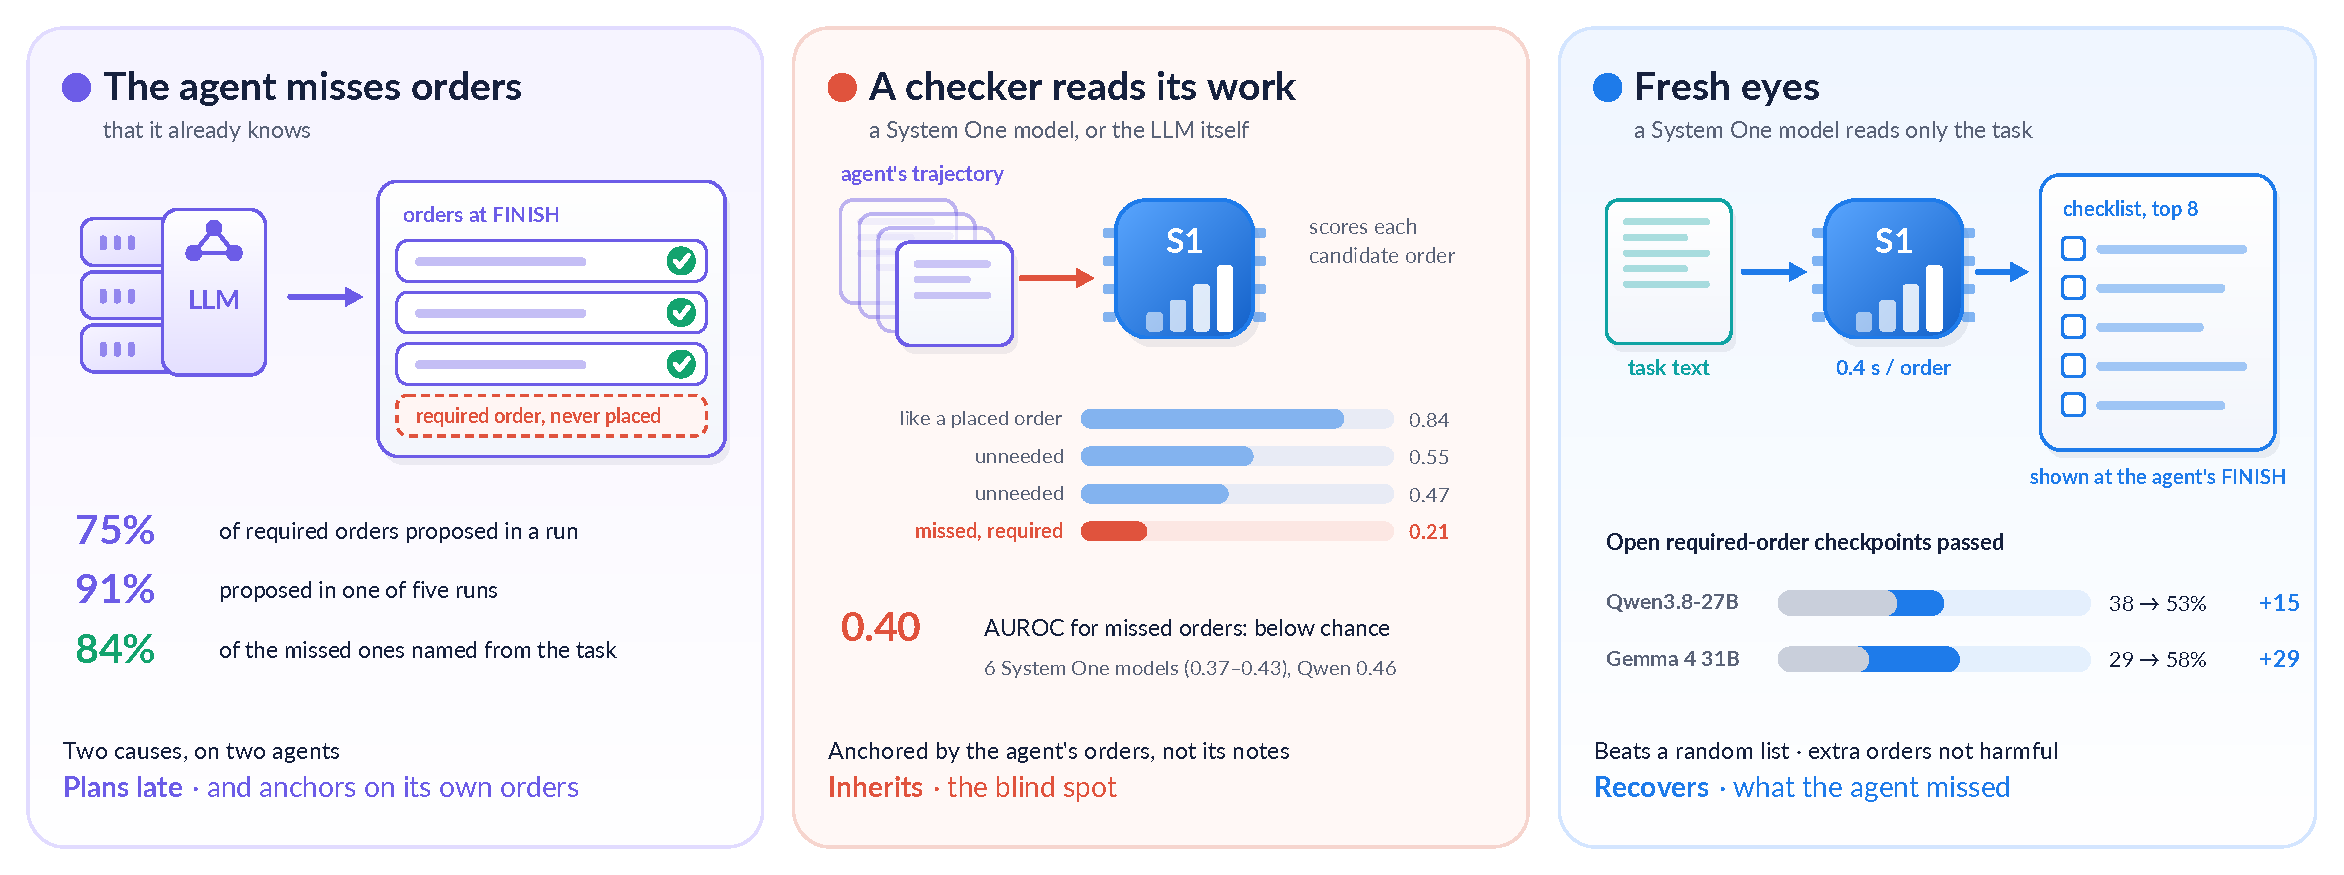
\includegraphics[width=\textwidth]{fig0_fresh.pdf}
\caption{\textbf{The paper in one figure.} \emph{Left:} a clinical agent finishes with a required order unplaced,
although the same model proposes it in other runs and names it from the task text alone (\S\ref{sec:know}). It plans
late and anchors on its own orders (\S\ref{sec:why}). \emph{Middle:} a checker that reads the agent's trajectory,
whether a System One model or the LLM, scores each candidate order largely by its resemblance to what the agent already
ordered, so the missed orders land below chance; reading only the task, the same models rank them above chance (mean
over six System One models; \S\ref{sec:inherit}).
\emph{Right:} a System One model that reads only the task ranks a checklist that, shown at the agent's finish,
recovers the missed orders for both agents (\S\ref{sec:fresh}). All numbers are aggregates; no patient data.}
\label{fig:story}
\end{figure*}

\section{Introduction}

A physician who has just finished a workup is the person least likely to spot what is missing from it. Medicine
answers this with second readers, consults and checklists: a fresh pair of eyes that has not followed the same path
\citep{croskerry2003cognitive,haynes2009checklist}. LLM agents now do physicians' work in the electronic health record.
They look up the problem list, pull the labs, order the workup and write the note \citep{physicianbench2026,yao2023react}.
We find that they miss orders for the same reason a physician does, that the usual machine remedy, a second model
reviewing the agent's work, fails in the same way, and that a second reader with genuinely fresh eyes recovers the
orders.

The missed orders are not gaps in knowledge. On PhysicianBench, 100 real outpatient consultations on a live FHIR
server, a Qwen3.8-27B agent proposes 75\% of the required orders in a single run but 91\% across five runs of the same
task, and given nothing but the task text it names 84\% of the orders its run went on to miss. Nor are they lost when
the agent chooses among its options: only 11\% of required orders are ever proposed and then not executed, while 19\%
are never proposed at all. Picking better among the agent's proposals, the idea behind best-of-$n$ selection and
verifiers, cannot reach them. The orders are lost earlier, while the agent generates what to do. Four findings follow,
on two agents from different model families (Qwen3.8-27B and Gemma 4 31B).

\paragraph{Agents plan late and anchor on their own orders} (\S\ref{sec:why}). Asking the agent to write its full
plan before its first order recovers orders it would otherwise miss for good; reminding it of the task does not. At
its finish, asking what is still missing works better when its own orders and notes are removed from view.

\paragraph{A reviewer that reads the agent inherits its blind spot} (\S\ref{sec:inherit}). Six System One decision
models, which score options in one forward pass, and the reasoning LLM itself rank the orders the agent missed
\emph{below chance} when they read its trajectory, and above chance when they read only the task. The anchor is the
agent's orders, not its notes or the chart. One fabricated order shifts the judgment, and telling the reviewer that
orders may be missing does not help. A reviewer scores each candidate by how much it resembles what the agent already
did.

\paragraph{Fresh eyes recover the orders} (\S\ref{sec:fresh}). A judge that reads only the task ranks a broad pool of
candidate orders before the run, and the agent sees the top eight when it first tries to finish. The pass rate of the
required-order checkpoints still failing at that point rises from 38\% to 53\% for Qwen and from 29\% to 58\% for
Gemma, more than with a random checklist from the same pool, and the orders it adds beyond the rubric are mostly
indicated or reasonable care.

\paragraph{One pass is enough} (\S\ref{sec:onepass}). The checker needs neither a special model nor reasoning. The
agent LLM without thinking ranks the checklist about as well as a System One model, and every slower way of asking
it, stating a probability, voting over samples or thinking for up to 8k tokens, ranks no better at up to a hundred
times the cost (Figure~\ref{fig:frontier}). What carries the fix is what the checker reads.

\medskip
We measure each intervention by \emph{branching}: every arm replays the same logged run up to the agent's first
finish and differs only from there, so that run-to-run noise, large in long agent runs, cancels. Every confirmatory
test was fixed in a dated log before its data existed. Appendix~\ref{app:path} tells the path that led here,
including the tests that did not hold.

\section{Setting}\label{sec:setup}

\paragraph{PhysicianBench} \citep{physicianbench2026} adapts 100 real outpatient consultations from 21 specialties into
long-horizon tasks on a FHIR server holding the records of 108 de-identified patients. Each task has 5--9
checkpoints (670 in total) of four types (data retrieval, clinical reasoning, action execution and documentation),
each graded by code or by an LLM judge. We use the released harness unchanged: a fresh server per task, the MiniAgent
loop with parallel tool calls and at most 100 steps, and the task's own graders. Our focus is the 92
\emph{required-order checkpoints} in 54 tasks: code-graded checks that a specific laboratory test, imaging study,
referral, procedure or medication was placed in the record. Some checkpoints require several orders, 118 in all. We
match an order to such a checkpoint with the grader's own name and code patterns. An order that matches none we call
\emph{outside the rubric}.

\paragraph{Agents.} The main agent is Qwen3.8-27B \citep{qwen38} with thinking on, in bf16 with 128k context. The
second is Gemma 4 31B-it, a different model family, with thinking on and FP8 weights, the precision at which one 128k
context fits beside the judge on our GPUs. It is a much weaker agent on this benchmark: it passes 51\% of checkpoints
against Qwen's 81\% and 8\% of tasks against 41\%, and places no order in 56\% of its runs. Both run in the same
harness, and the grader's judge is Qwen with thinking off for every arm.

\paragraph{Judges.} \emph{System One} decision models, named after the fast mode of human judgment
\citep{kahneman2011thinking}, take a state, a typed question and named options and return a probability per option in
one forward pass \citep{typesafe2026jev,clef2026}. We use six open ones of the agents' own scale (26--31B parameters):
Clef-27B \citep{clef2026}, pplx-decider-v1.2 (pplx12), d3, linne-oak-1.0, amos-1-large and decider-31b, each served
with its authors' code at a pinned revision (Appendix~\ref{app:interface}). The LLM answers the same request either
with thinking on or in one pass, with P(Yes) read from its first-token probabilities. Everything runs locally on one
node; no record leaves it (\S\ref{sec:ethics}).

\paragraph{Branching from a shared prefix.} For an intervention at the agent's finish we take each logged run whose
first \textsc{finish} leaves a required-order checkpoint \emph{open} (still failing): 51 cases for Qwen and 65 for
Gemma. Every arm replays that run's turns against a fresh environment up to the \textsc{finish} and branches there.
The \emph{none} arm keeps the logged finish; replaying it reproduces 99.7\% (Qwen) and 99.6\% (Gemma) of the logged
checkpoint outcomes. The other arms run 3--5 times each. The primary outcome is the pass rate of the checkpoints that
were open at the branch. Forbidden orders, which the rubric also lists, occurred in no arm. Differences are paired
over cases with 95\% bootstrap intervals.

\begin{figure*}[t]
\centering
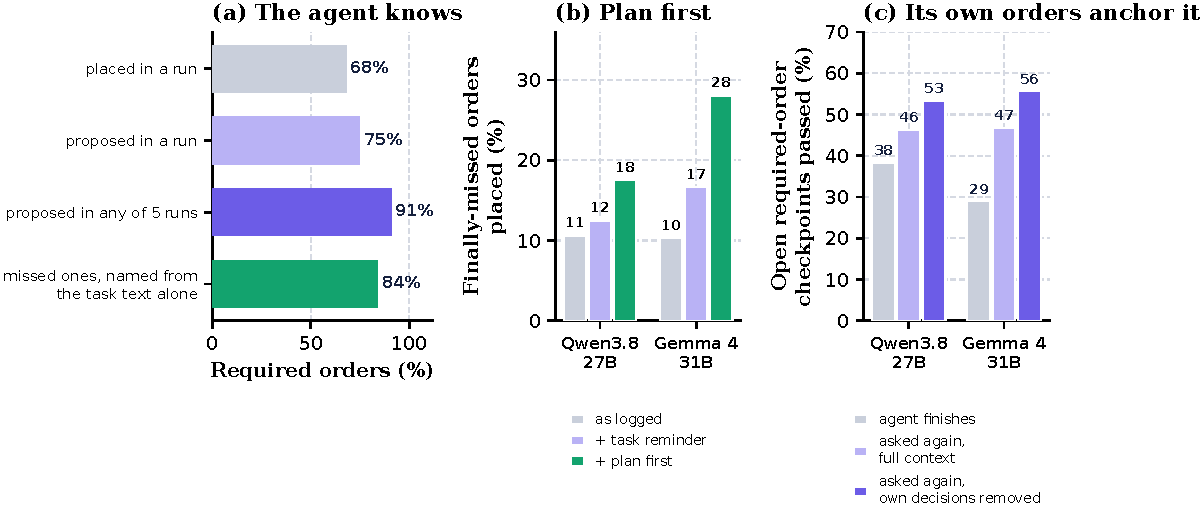
\includegraphics[width=\textwidth]{fig7_why.pdf}
\caption{\textbf{Why the agent misses orders.} (a) Qwen3.8-27B knows the orders it misses: share of required orders
placed and proposed in a single run (mean over five logged runs), proposed in any of the five (54 tasks, 590 order
$\times$ run pairs), and the share of the
orders its run left open that Qwen names from the task text alone (26 tasks, 36 orders). (b) It plans late: at the
first order step, replayed with $K{=}5$ samples, the share of the orders the run finally missed that the agent places,
as logged, after a reminder of the task, and after being asked to write its full plan first (Qwen 48 cases, Gemma 18). (c) It anchors on its own orders: at its first finish, the share of open required-order
checkpoints that pass when the agent finishes as logged, when it is asked for the missing orders with its full
context, and when it is asked with its own decision turns removed (Qwen 51 cases $\times$ 5 runs, Gemma 65 cases
$\times$ 3 runs).}
\label{fig:why}
\end{figure*}

\section{The agent knows the orders it misses}\label{sec:know}

If the agent lacked the knowledge, no amount of re-reading would help. It does not lack it. We pooled the orders
proposed by any sample in five logged runs of each task: the LLM's own run and four runs in which a System One model
took part in its decisions (Appendix~\ref{app:path}). On average a single run proposes 75\% of the required orders and
places 68\%; the five runs together propose 91\% (Figure~\ref{fig:why}a). Of the required orders a run never
proposes, 62\% are proposed in another run of the same task. A second test asks directly. Qwen, without thinking and
given nothing but the task text, lists the orders that could be indicated, eight samples per task. Its list covers
84\% [71, 95] of the required orders that the agent's own run left open at its finish. The model that failed to place
these orders while working in the chart names them readily from the request alone.

The orders are lost at generation, not at choice. The agent samples five candidate turns at every step; following
each of the 118 required orders along its trajectories, it places 69\%, only 11\% are proposed at some step and never
executed, and 19\% are never proposed by any sample at any step. A selector, however good, can recover at most the
11\%. Putting System One models in the agent's decision seat to choose among its proposals indeed kept the agent's
level without raising it (Appendix~\ref{app:path}). What fails is the step from knowing to doing.

\section{Why it misses them: it plans late, and it anchors on its own orders}\label{sec:why}

\paragraph{Acting before the plan is written.} One explanation is drift: over a long trajectory of record lookups the
agent loses track of the task. Another is that it starts ordering before it has enumerated what the task needs, and
what it never enumerates it never orders. Drift predicts that a reminder helps; late planning predicts that a plan
does. We replayed the agent's first order step with five samples under three conditions: as logged, with the task
instruction repeated, and with a request to write the full assessment and plan, listing every order the task
requires, before placing any (Figure~\ref{fig:why}b). For Qwen a reminder moves orders earlier but not into the final
record; for Gemma it does neither. Planning first does both. For Qwen, the share of the run's finally missed orders
placed at that step rises from 11\% to 18\% (+7 points [2, 13]), against +2 [$-$2, +5] for the reminder. For Gemma it
rises from 10\% to 28\% (+18 [4, 32]) and beats the reminder by +11 [2, 23]. Forgetting the task affects when orders
are placed; the orders lost for good are those the agent commits past before its plan exists.

\paragraph{Anchoring on its own orders.} At the agent's first finish we asked for the missing orders in two ways
(Figure~\ref{fig:why}c). Both arms ask the same question, ``place every order that this task requires and that has
not been placed yet''. One asks it with the agent's full context. The other asks it with every decision turn removed:
no orders, messages or notes, only the task and the chart the agent retrieved. Asking at all helps: open required
checkpoints rise from 38\% to 46\% for Qwen (+8.0 [2.6, 15.1]) and from 29\% to 47\% for Gemma (+17.8 [10.6, 25.7]),
so the agent can still produce the orders. Asking without its own decisions in view helps more: +7.1 [1.0, 13.7]
points over the full context for Qwen and +8.9 [3.2, 15.3] for Gemma, with no loss over all checkpoints. The agent's
record of what it has done suppresses orders that it can still generate. Both effects are larger for the weaker
agent.

\begin{figure}[t]
\centering
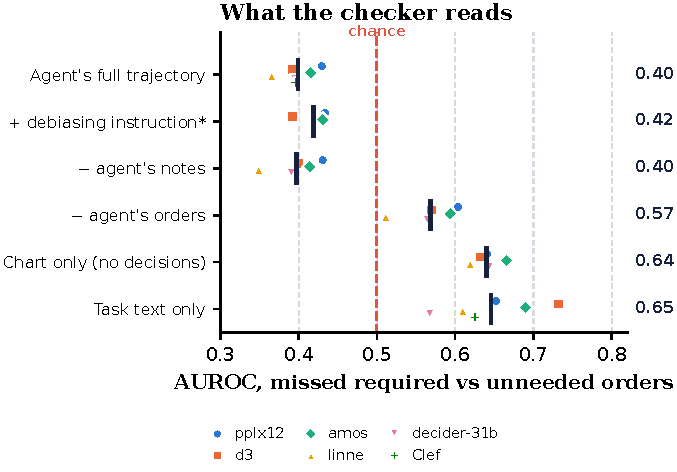
\includegraphics[width=\columnwidth]{fig6_anchor.pdf}
\caption{\textbf{A checker that reads the agent inherits its blind spot.} AUROC of each System One model for telling
the required orders the agent missed from unneeded candidate orders (21 tasks with a missed required order), by what
the checker reads: the agent's trajectory at its finish; the same with a debiasing instruction (*three models); without
the agent's notes; without its orders; the retrieved chart with no decisions; the task text alone. Black line: mean
over the models shown in the row.}
\label{fig:anchor}
\end{figure}

\section{A reviewer that reads the agent inherits its blind spot}\label{sec:inherit}

The standard remedy for an agent's omissions is review: a second model reads the agent's work and flags what is
missing, as in self-refinement and LLM-as-judge pipelines \citep{madaan2023selfrefine,zheng2023judge}. A System One
model is an attractive reviewer here. It scores a candidate order for a patient in one forward pass, so it can screen
dozens of candidates where an LLM would deliberate over a few. We tested this at the agent's first finish. The
candidates are every order proposed in the task's five runs that the agent has not placed (about 44 per task). Each
checker scores each candidate with the question ``is this order indicated for this patient as part of completing the
task?''. The measure is how well it separates the required orders the agent missed from the unneeded ones (AUROC, per
task).

\paragraph{Reading the trajectory, every checker ranks the missed orders below chance.} With the agent's trajectory
as input, all six System One models score 0.37--0.43 (Figure~\ref{fig:anchor}). Given only the task text, the same
models score 0.57--0.73, a paired gain of +0.17 to +0.34 with every interval excluding 0. The reasoning LLM is no
exception: Qwen with thinking goes from 0.46 to 0.62 on the same questions (+0.17 [0.07, 0.27]). The anchoring is what
happens to any judge that reads the agent's actions, not a quirk of small decision models. The trajectory hurts even
on the orders the agent did place (0.65--0.72 with it, 0.74--0.86 without).

\paragraph{The anchor is the agent's orders.} Removing only the agent's decision turns (orders, messages, notes) and
keeping the full chart it retrieved brings the checker back to about its task-only level (0.62--0.67; +0.21 to +0.25
over the trajectory). The chart does not mislead the checker; the agent's decisions do. Among the decisions, the
orders carry 57--83\% of the recovery and the notes none ($-$0.07 to +0.04). A causal test confirms the direction:
inserting one fabricated step in which the agent places the candidate order raises the checker's P(Yes) by +0.07 to
+0.10, for required and unneeded orders alike.

\paragraph{The mechanism is plan conformity.} With the trajectory, a checker's score tracks how closely the candidate
resembles the agent's placed orders (within-task Spearman 0.28--0.38 for System One models, 0.47 for Qwen; 0.05 with
the task text). The missed orders resemble the agent's placed orders less than unneeded candidates do (name overlap
0.26 against 0.34), so similarity alone ranks them below chance (AUROC 0.41). A checker that reads the agent's work
grades candidates by their conformity to that work, so it inherits exactly the agent's omissions.

\paragraph{An instruction does not fix it; the input must change.} Adding ``the agent may have missed orders; judge
each one independently'' recovers 1--6\% of the gap for System One models and 8\% for Qwen. The models read the
sentence, since their P(Yes) rises across the board, but the ranking does not change.

\begin{figure*}[t]
\centering
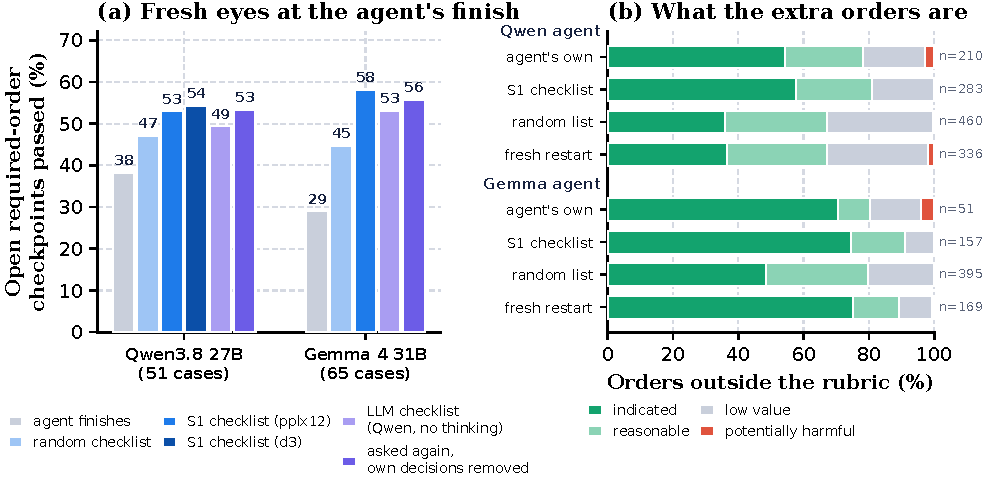
\includegraphics[width=\textwidth]{fig8_loop.pdf}
\caption{\textbf{Fresh eyes in the loop.} (a) At each agent's first finish, from the same replayed prefix: the share of
open required-order checkpoints that pass when the agent finishes as logged; when it sees eight orders drawn at random
from the task-prior pool; when it sees the eight ranked highest from the task text by pplx12 (both agents) or
d3 (Qwen only), or by the agent LLM Qwen without thinking from the same request (both agents); and, for reference, the fresh-context restart of Figure~\ref{fig:why}c. Qwen: 51 cases $\times$ 5 runs
(d3 and the LLM checklist: 3); Gemma: 65 cases $\times$ 3 runs. (b) What the orders outside the rubric are: each order rated alone by a blinded LLM judge (Gemma 4)
that sees the task and the retrieved chart. Bars give the share of distinct orders per case by source; n is the number
of orders rated.}
\label{fig:loop}
\end{figure*}

\section{Fresh eyes: a checklist from the task}\label{sec:fresh}

The findings fix the design. The checker reads the task, not the agent's work (\S\ref{sec:inherit}). Candidates come
from a broad pool, because the agent knows the orders but does not reach them in one pass (\S\ref{sec:know}). The
intervention comes when the agent's own plan is complete and it is about to stop (\S\ref{sec:why}). The agent keeps
the decision.

\paragraph{Design.} Before the run, the LLM without thinking reads the task text and lists candidate orders: eight
samples of up to 15 each, merged by name, about 67 per task (the \emph{task-prior pool}). A System One model scores
every candidate from the task text alone. At the agent's first finish, candidates already placed are dropped, and the
top eight are shown with one instruction: ``Check each against the chart and the task. Place any that are indicated,
and only those, then finish.'' (Appendix~\ref{app:prompts}). The ranking costs one forward pass per candidate and is
computed before the run starts.

\paragraph{It recovers the missed orders, for both agents.} From the same prefix, the checklist raises open
required-order checkpoints from 38\% to 53\% for Qwen (\up{14.7} points [6.7, 24.1]) and from 29\% to 58\% for Gemma
(\up{29.2} [20.0, 39.5]) (Figure~\ref{fig:loop}a). The ranking matters: it beats eight orders drawn at random from the
same pool by +5.9 [0.6, 11.8] for Qwen and +13.6 [6.5, 21.7] for Gemma. A second System One ranker, d3, does as well
(54\% for Qwen; +7.2 [1.1, 13.3] over the random list). The checklist matches restarting the agent with its own
decisions removed (\S\ref{sec:why}; $-$0.4 and $-$2.6 points, both n.s.): two routes to the same fix, changing what is
read before the agent stops. Over all checkpoints, not only the open ones, the pass rate rises by 4.7 points for Qwen
and 7.8 for Gemma.

\paragraph{The extra orders are reasonable care.} The checklist also adds about 1.5 orders per case that no rubric
item names, fewer than the random list (2.0 and 2.3). PhysicianBench neither credits nor penalises such orders, so we
asked what they are. A blinded LLM judge (Gemma 4) saw the task and the retrieved chart and rated each order alone,
without its source, as indicated, reasonable, low value or potentially harmful (Figure~\ref{fig:loop}b). 81\% of the
checklist's extra orders for the Qwen agent and 91\% for the Gemma agent are indicated or reasonable, at least the
rate of the agents' own extra orders (78\%, 80\%) and above the random list's (67\%, 80\%). None was rated
potentially harmful, against 2.9\% and 3.9\% of the agents' own. A second judge, Qwen, agrees in direction. What the
rubric counts as excess is mostly care it does not list.

\begin{figure}[t]
\centering
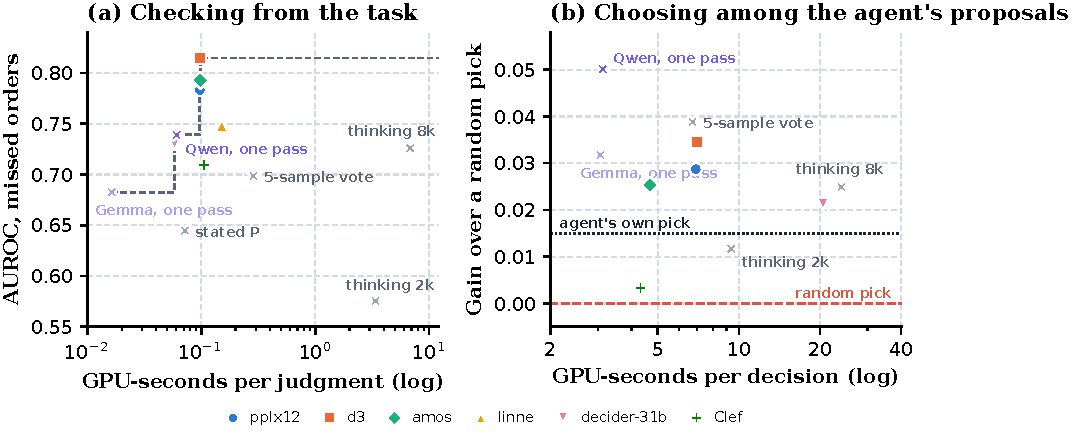
\includegraphics[width=\columnwidth]{fig9_frontier.pdf}
\caption{\textbf{One pass is enough.} Each judge scores the task-prior pool from the task text alone. AUROC of the
orders the agents left open at their first finish (133 cases in 42 tasks; the two thinking budgets on a seeded 15 of
them) against GPU-seconds per judgment on one H100 with 8 concurrent requests. Coloured: System One models; crosses:
the LLMs. Dashed: the frontier, off which a judge falls when a cheaper one ranks better (paired 95\% interval
excluding 0). Appendix~\ref{app:frontier} gives every interval and the selector role.}
\label{fig:frontier}
\end{figure}

\section{One pass is enough}\label{sec:onepass}

\paragraph{No special model.} Does the checker need a System One model? We let the agent LLM, Qwen without thinking,
rank the same pool from exactly the System One model's request, reading P(Yes) from its first-token probabilities.
Its checklist works too: \up{11.1} points [4.3, 19.6] for the Qwen agent and \up{24.2} [15.5, 33.0] for Gemma over
the agent's finish, within a few points of the System One list (+3.6 [$-$1.1, 8.0] and +5.0 [$-$2.6, 13.2] in
pplx12's favour). Pooling models does not help either: a committee of all six System One models, their ranks
averaged, does no better than one.

\paragraph{No reasoning.} Figure~\ref{fig:frontier} places every judge by quality and cost: how well it ranks the
orders the agents left open, against its GPU time per judgment. One-pass judgments, System One models and the LLM's
first-token probability, form the frontier. Thinking with an 8k-token budget ranks no better than the LLM's one pass
at 112 times the GPU time; with 2k tokens it mostly runs out of budget. A stated probability and a vote over five
samples rank worse. The three best System One models (d3, amos, pplx12) rank above the LLM's one pass by 0.04--0.08 at
1.6 times its cost, and System One probabilities are better calibrated (Brier 0.16--0.28 against 0.29--0.50); the six
on average are level with it. What carries the fix is what the checker reads, not which model reads it or how long
it thinks.

\section{Related work}

\paragraph{Self-correction and review.} Agents and LLMs are often asked to critique and revise their own output
\citep{madaan2023selfrefine,shinn2023reflexion}, and reasoning errors are hard to self-correct without external
signal \citep{huang2024cannot}. LLM judges favour their own generations \citep{panickssery2024selfpref}. We locate a
specific failure of review inside an agent loop. A reviewer that reads the agent's work, whether it is the agent
itself, another LLM or a System One model, scores candidates by their conformity to that work. Changing what the
reviewer reads fixes it; instructions and reasoning do not.

\paragraph{Anchoring and premature closure.} Anchoring on an initial estimate \citep{tversky1974heuristics} and
premature closure are among the most cited cognitive errors in clinical diagnosis, and fresh perspectives and
checklists are the classic remedies \citep{croskerry2003cognitive,haynes2009checklist}. We find the agent-level
analogue: the agent anchors on the orders it has placed, and so does anything that reads them. Planning before
acting \citep{wang2023planandsolve} also helps here, though it does not close the gap.

\paragraph{Choosing among samples.} Self-consistency \citep{wang2023selfconsistency}, trained verifiers
\citep{cobbe2021verifiers} and process reward models \citep{lightman2024verify} pick among sampled outputs. Our
analysis of where required orders are lost shows why selection has little to gain when the missing content is never
sampled.

\paragraph{System One models and clinical agents.} JEV introduced the typed-question interface that System One models
answer in one forward pass \citep{typesafe2026jev}; Clef is an open 27B model of this kind \citep{clef2026}. They
approach frontier LLMs as judges \citep{li2026jevjudge}, and as selectors in general agents most of their wrong
actions follow a correct reading of the state \citep{li2026reading}. PhysicianBench \citep{physicianbench2026} grades
physician tasks in a live record system and has been run only with generative agents. We find that the useful place
for a one-pass judge in a clinical agent is beside the agent, reading the task, not in its decision seat.

\section{Discussion}

\paragraph{Design rules.} Three rules follow, and none is specific to one model. \emph{Check the task, not the
agent:} a reviewer, human or model, should read the request and the chart, not the agent's decisions, because the
decisions pull its judgment toward conformity. \emph{Plan before acting, review before finishing:} the agent loses
orders by committing before the plan exists and by stopping once its own orders look complete. \emph{Screen broadly
in one pass:} a one-pass judge, a System One model or the LLM without thinking, scores dozens of candidates from the
task in seconds, while the LLM generates the candidates and keeps the decision; reasoning adds cost, not accuracy.

\paragraph{What System One models made possible.} Six independently trained one-pass judges, each asked the same
question with and without the agent's work, let us run the input ablations of \S\ref{sec:inherit} over thousands of
judgments and show that the anchor is not a quirk of one model. In deployment they are a ready-made checker that
returns a calibrated probability per option. Their place is beside the agent, reading the task.

\paragraph{The anchor is general.} The checker in \S\ref{sec:inherit} and the agent in \S\ref{sec:why} fail in the same
way: both score what to do next by what has already been done. The agent's restart and the checker's input ablation
are the same intervention, removing the agent's decisions from view, and they help both. We expect this to hold for
agents that act in other record systems and other domains wherever omissions matter: software changes, audits,
procurement.

\section*{Limitations}

We study one benchmark of outpatient consultations with two agent LLMs of similar scale; the second, in FP8, is much
weaker, and all comparisons are within one agent. The rubric names one acceptable set of orders; our ratings of
orders outside it come from two LLM judges with moderate agreement ($\kappa$ 0.48--0.49), not physicians. The grader's
judge is the local Qwen model shared by every arm, so absolute scores are not comparable with the leaderboard.
Online effects are measured from shared prefixes at the agent's first finish; an end-to-end deployment that combines
planning first with the checklist remains to be run. Costs are measured on each model's own serving stack.
Appendix~\ref{app:prereg} lists every pre-registered test, including those that failed.

\section*{Ethics and data}\label{sec:ethics}

PhysicianBench's records are real de-identified patients under a data use agreement. All models run locally, a socket
guard blocks any non-local connection from agent and grader processes, and trajectories, notes, candidate orders and
judge ratings stay on access-controlled storage outside version control. We report aggregates only. The checklist is
a screening aid shown to an agent that keeps the decision. In deployment, a clinician would review every order.

\bibliography{refs}

\appendix

\section{The path to fresh eyes}\label{app:path}

The main text presents the result. This appendix records how we reached it, including what did not work;
Appendix~\ref{app:prereg} lists every pre-registered test with its verdict.

\paragraph{We began in the decision seat.} System One models read a state and options and return a probability for
each in one forward pass, and choosing among options is what an agent does at every step. So we first put them in the
agent's decision seat (Appendix~\ref{app:seat}). In \sel{} the LLM proposes five complete next turns and the System
One model picks one; in \tool{} it picks the kind of action and the LLM writes the call. Choosing among proposals,
Clef keeps the LLM's level (80.2\% of checkpoints against 81.3\%; task success $-$4 points, $p=0.52$). Choosing the
action itself, it breaks the agent (7\% of tasks pass): it acts after little retrieval and rewrites the note again and
again. All six models share a \emph{commitment bias}: on a fixed exam of 1,460 logged decisions they pick ordering
turns 1.3--1.6$\times$ and finishing turns 1.3--1.4$\times$ as often as the LLM. pplx12's early gain on required orders
(+13 points on its first 76 tasks) failed a pre-registered replication on the 24 it had not run ($-$18 [$-$36, $-$2]),
and a decider consulted only at order steps added orders, mostly outside the rubric, without adding required ones.
Table~\ref{tab:ceiling} shows why no selector could do much: the required orders are lost at generation. A last,
pre-registered test of the selector role continued every option of 60 decisions to the agent's finish (539 graded
runs; Appendix~\ref{app:frontier}). No judge beat the agent's own pick reliably, and the agent LLM's own first-token
choice beat the System One average ($-$2.6 points [$-$6.3, $-$0.1]). That moved the question from \emph{who decides}
to \emph{why the agent never proposes what it needs}.

\begin{table}[t]
\centering\small
\begin{tabular}{@{}lrrr@{}}\toprule
Required orders (\%) & \llm{} & Clef & pplx12 \\\midrule
Placed & 69 & 64 & 72 \\
Proposed, never executed & 11 & 8 & 4 \\
Never proposed & 19 & 28 & 24 \\\midrule
Step omissions placed later & 79 & 13 & 25 \\\bottomrule
\end{tabular}
\caption{\textbf{Where required orders are lost,} along each decision maker's own trajectories (54 tasks, 118
required orders; Clef and pplx12 in \sel). The middle row is the most any selector could recover; the agent's real
loss is the orders it never proposes.}
\label{tab:ceiling}
\end{table}

\paragraph{Noise taught us to branch.} Two runs of the same agent differ on 28 of 100 tasks. Tested on independent
runs, the task-prior checklist separated neither from a random checklist (+0.045 [$-$0.07, 0.19]) nor from an
independent baseline run ($-$0.02, n.s.). Branching from a shared prefix, which cancels the run-to-run variation,
measured its effect; every online result in the main text uses it.

\paragraph{Designs that did not work.} A richer chart did not help a trajectory-reading screener on the orders the
agent never placed (AUROC 0.44). A checklist drawn from the orders proposed during the run and ranked by a System One model did
not beat the same pool ranked by proposal frequency ($-$0.02 [$-$0.15, 0.11]); the pool, not the ranking, was too
narrow. Showing the ranker the orders already placed, to avoid repeats, halved its top-3
coverage of the open orders (0.31 to 0.15), and so did a factorized ranking with a separate repeat judge. This is how
we first saw that the agent's orders anchor any judge, and why the final design shows the ranker the task alone and
removes repeats afterwards. Offline, a nudge and a fresh question at the finish helped, but by less than the bars we
had set (+0.08 and +0.07 against 0.15 and 0.10), and the misses an agent's own note mentions were mostly not false
claims of completion (0.40).

\paragraph{Results short of their pre-registered bars.} One fabricated order raises the checker's P(Yes) by +0.07 to
+0.10: the predicted direction, short of the +0.15 we set. Removing the agent's decisions recovers Qwen as a checker
by +0.12 [$-$0.005, 0.26], like the System One models' recovery in size but with an interval touching 0. The checklist
adds more orders outside the rubric than the +1.0 per case we allowed (+1.47 for Qwen, +1.56 for Gemma), which is why
we asked what they are (\S\ref{sec:fresh}). Rated as one list per case, where near-duplicate variants sit side by
side, no checklist order is harmful, but the checklist's orders are no less appropriate than the agent's own for only
one of the two agents; rated alone, as in the main text, they are for both. Two tests asked whether System One models
beat the LLM: a committee of six against the LLM ranker (+1.9 points [$-$2.7, 6.4], no), and System One training
against the same LLM read out in one pass, as checker and as selector (level on average and behind;
Appendix~\ref{app:frontier}).

\paragraph{Beyond orders.} The agents differ in their other failures, less alike than we predicted (one of three
error types matched). Labelled by the local LLM, Qwen's failed clinical-reasoning and documentation checkpoints are
most often \emph{wrong} content (wrong judgments in reasoning, 70\% of the wrong items; misstated facts in notes,
62\%), while Gemma's are most often \emph{incomplete}. When Gemma's note mentions an order it never placed, 60\% of the
time it is a recommendation it did not carry out (Qwen: 10\%). The error profile depends on the agent; the two
mechanisms behind missed orders, and the remedies that follow from them, hold for both.


\section{Decision interface}\label{app:interface}

\paragraph{Questions.} The System One model receives the state and one Choice question. For \sel{}: \emph{``The state
shows a clinical task assigned to an AI agent that works in an electronic health record through FHIR tools, followed
by the agent's actions and their results so far. Each option is a candidate next action for the agent. Choose the
candidate that best advances completing the task correctly, completely and safely.''} For \tool{} the second and third
sentences read: \emph{``Each option is a tool the agent can use for its next action, or finishing with a final answer.
Choose what the agent should do next to complete the task correctly, completely and safely.''} Options are the
rendered turns (\sel) or each tool's name with the first paragraph of its description, plus \textsc{finish} (\tool).

\paragraph{State.} The state is the task instruction followed by every step: the action, rendered as tool calls with
full arguments, and its results as the LLM saw them. It is fitted into the System One model's 32,768-token context
deterministically: tool results are kept in full, then shortened oldest-first to 800 characters, then omitted
oldest-first, each by the smallest number that fits. In the \sel{} run \DECSelshort\% of decisions saw shortened
results and \DECSelomit\% saw omitted ones.

\paragraph{Other System One models.} pplx-decider-v1.2 (\texttt{cce0f3f8}), d3 v3.1.0 (\texttt{cbff3a3c}),
linne-oak-1.0 (\texttt{20da7bf3}), amos-1-large (\texttt{d67e051c}) and decider-31b (\texttt{e12ddf20}) each run their
authors' own serving code on H100 GPUs, locally and offline. pplx-decider-v1.2 ships a library only, which we call on
its reference path. decider-31b is NVFP4, which an H100 runs through vLLM's weight-only FP4 path; its authors used
Blackwell GPUs. linne-oak-1.0 needs two GPUs for 32k-token inputs. Every model receives the state and question built
for Clef, with the same fitting rule, counted in its own tokenizer. Five exam questions whose options alone exceed the
32k window are unanswerable for every model.

\paragraph{The LLM.} Qwen3.8-27B with thinking on, temperature 1.0, top-$p$ 0.95, top-$k$ 20, at most 16,384 completion
tokens per call. Identical replicas serve all arms; each task is routed whole to the less loaded replica, independent
of the arm.

\FloatBarrier
\section{Prompts}\label{app:prompts}

\paragraph{Task-prior pool (LLM, no thinking, eight samples).} \emph{``A clinical task assigned to an AI agent that
works in a patient's electronic health record: [task]. Without seeing the chart, list the orders (laboratory tests,
imaging, referrals or consults, procedures, medications) that could be indicated as part of completing this task. Up
to 15, one per line, each in the form ServiceRequest: <name> (code <code>) or MedicationRequest: <name> (code <code>),
leaving out the code part when unsure. Nothing else.''}

\paragraph{System One screening question.} The state is the task instruction alone (task-only) or the agent's
trajectory; the options are Yes and No: \emph{``Consider this order for the patient: [order]. Is this order indicated
for this patient as part of completing the task (whether or not the agent has already placed it)?''} The score is
P(Yes).

\paragraph{Checklist at the finish.} \emph{``Before you finish: a screening model reviewed orders that came up while
working on this task and flagged these as possibly indicated for this patient and not yet placed: [eight orders].
Check each against the chart and the task. Place any that are indicated, and only those, then finish.''}

\paragraph{Restart at the finish (full and fresh context).} \emph{``Based on the task and the patient data gathered so
far, place every order that this task requires and that has not been placed yet, then finish.''} In the fresh arm,
every assistant turn that calls an order, message, appointment or note tool, and the tool results answering it, are
removed; the system prompt, the task and all retrieval turns remain. Only order calls are executed, minus repeats of
placed orders.

\paragraph{First order step.} Reminder: \emph{``Reminder of your task: [task instruction]''}. Plan first:
\emph{``Before placing any orders, write out your full assessment and plan in your reply, listing every order the
task requires. Then place every order in that plan.''}

\paragraph{Order appropriateness (judges).} The judge sees the task and the retrieved chart (the fresh context above)
and one candidate order, and answers one letter: A indicated (standard of care for the patient's current problem); B
reasonable (a defensible addition a careful physician might order); C low value (unnecessary, not supported by the
data, or unrelated to the task); D potentially harmful (contraindicated, a wrong drug or dose for this patient, or risk
clearly exceeding benefit). Thinking on, temperature 0. The pre-registered version rated each case's orders in one
list; rated in a list, near-duplicate variants of one order sit side by side and later copies are marked low value, so
we report the single-order ratings in the main text, and the list version (in which no checklist order is rated
harmful either) in the research log.

\FloatBarrier
\section{The cost--quality frontier of one-pass judges}\label{app:frontier}

\begin{table}[t]
\centering\small
\setlength{\tabcolsep}{2.5pt}\begin{tabular}{@{}lrrrr@{}}\toprule
 & \multicolumn{2}{c}{Checker} & \multicolumn{2}{c}{Selector} \\
Judge & AUROC & GPU-s & gain & GPU-s \\\midrule
d3 & \textbf{0.815}$^*$ & 0.10 & 0.035$^*$ & 7.0 \\
amos & 0.793$^*$ & 0.10 & 0.025$^*$ & 4.7 \\
pplx12 & 0.783$^*$ & 0.10 & 0.029$^*$ & 6.9 \\
linne & 0.748 & 0.15 & 0.032 & OOM \\
decider-31b & 0.730$^*$ & 0.06 & 0.021 & 20.5 \\
Clef & 0.709 & 0.11 & 0.003 & 4.3 \\\midrule
A, Qwen first-token & 0.739$^*$ & 0.06 & \textbf{0.050}$^*$ & 3.1 \\
A-G, Gemma first-token & 0.682$^*$ & 0.02 & 0.032$^*$ & 3.1 \\
B, stated P & 0.645 & 0.07 & -- & -- \\
D, 5-sample vote & 0.699 & 0.29 & 0.039$^*$ & 6.7 \\
C2, thinking 2k & 0.576 & 3.38 & 0.012$^*$ & 9.4 \\
C8, thinking 8k & 0.726 & 6.82 & 0.025$^*$ & 24.0 \\
Agent's own pick & -- & -- & 0.015 & 0 \\\bottomrule
\end{tabular}
\caption{\textbf{One-pass judges against every way of asking the LLM.} $^*$ on the cost--quality frontier. Checker:
AUROC of the open required orders; selector: gain in share of checkpoints over a random pick. Checker C2 and C8 on 15
tasks. OOM: on one H100, linne's server ran out of memory with 8 concurrent selector states of up to 32k tokens
(it needs two GPUs for such inputs, Appendix~\ref{app:interface}), so it has no selector cost. At this power most selector judges are not separable, so the selector frontier is wide.}
\label{tab:frontier}
\end{table}

This test (pre-registered as F) asks whether the training that makes a System One model makes it a better judge than
an LLM of the same scale used in every reasonable way, at the same measured cost, in two roles. Every judge gets the
same instruction, question, options and option letters. The LLM configurations are Qwen3.8-27B unless stated.
\emph{A}: no thinking, the System One request as a lettered choice, the distribution from the first token's
log-probabilities; \emph{A-G} the same with Gemma 4 31B, the base family of linne and decider-31b. \emph{B} (checker
only): no thinking, one line `P=<0-100>'. \emph{C2, C8}: thinking on, at most 2,048 or 8,192 generated tokens, then the
answer; no answer counts as 0.5 (checker) or the agent's own pick (selector). \emph{D}: no thinking, five samples at
the default temperature, the share of Yes or the majority letter. Cost is GPU-seconds per judgment on one H100 with 8
concurrent requests after a warm-up (checker: 200 seeded pool items; selector: 45 questions), each model on its own
serving stack. A judge is on the frontier unless another has a higher score, with the paired 95\% interval over tasks
excluding 0, at no higher cost.

\paragraph{Checker.} Items are the 3,576 task-prior pool orders, scored from the task text alone. For each logged run's
first finish (Qwen runs 1 and 3, Gemma runs 1 and 2; 133 cases in 42 tasks) we take the AUROC of pool orders matching
an open required order against orders matching none, averaged within and then over tasks. C2 and C8 ran on a seeded 20
tasks (15 with a case) and are compared on those only.

\paragraph{Selector.} 60 exam decisions (the agent's five sampled next turns, differing in kind or in the orders
placed; at most two per task). Each option is executed from the replayed state and the agent continues to its finish,
twice (once for a finish option); an option's value is its mean share of checkpoints passed (539 graded runs). On the
37 decisions whose options differ in value, a judge's gain is the value of its pick minus the mean option value.

\paragraph{Readings.} As checker, the six System One models on average are level with A (+0.024 [$-$0.008, 0.057]);
three are above it (d3 +0.076 [0.033, 0.120], amos +0.054 [0.011, 0.096], pplx12 +0.044 [0.001, 0.086]). The
Gemma-family pair beats Gemma's own read-out (+0.057 [0.007, 0.108]). The System One mean beats a stated probability
(+0.118 [0.070, 0.167]) and the vote (+0.065 [0.027, 0.101]) and is level with thinking at 8k (+0.046 [$-$0.004,
0.098]), which costs 112$\times$ A. The frontier is A-G, decider-31b, A, pplx12, d3 and amos; B, D, C2, C8, Clef and
linne are off it. As selector, the System One mean trails A ($-$0.026 [$-$0.063, $-$0.001]) and is level with thinking,
the vote and the agent's own pick; no judge beats the agent's own pick reliably (A +0.035 [$-$0.011, 0.089]). By the
readings fixed in advance, System One training is not a reliable edge over the same LLM read out in one pass in
either role, and no costlier way of asking the LLM reliably beats its one-pass read-out in either role.

\FloatBarrier
\section{Pre-registered tests}\label{app:prereg}

Every confirmatory test was written into a dated research log, with its prediction and bar, before any of its data
existed; amendments were logged before results were seen. Table~\ref{tab:prereg} lists them in the order run. Tests
that failed shaped the study as much as those that held: P1, P9 and O1 moved us from independent runs to
shared-prefix branching, the unplaced-order breakdown of P6 led to the task-only screen, and P8b and P10 kept the
agent's orders out of the ranker.

\begin{table*}[t]
\centering\small
\begin{tabular}{@{}p{0.07\textwidth}p{0.45\textwidth}p{0.27\textwidth}l@{}}\toprule
Test & Prediction & Result & Verdict \\\midrule
P1 & pplx12's \sel{} gain on required orders replicates on 24 unseen tasks & $-$18 points [$-$36, $-$2] & fails \\
P2$'$ & orders-only gate: required-order gain, notes at the LLM's level & +5 [$-$2, 14]; notes, steps restored & primary fails \\
P3 & a consequential exam key ranks deciders as online & 11 questions, too few & not supported \\
P4 & blind decider picks like the informed one (style only) & agreement 41\% & rejected \\
P5 & gate places more orders, more outside the rubric (replication) & +0.61 [0.12, 1.13]; +0.35 n.s. & half holds \\
P6 & a System One screener reading the agent's state ranks required orders & AUROC 0.74 (unplaced: 0.43, post hoc) & holds \\
P6b & a richer chart helps on the unplaced orders & 0.44 & fails \\
P6c & a task-only screener ranks the unplaced orders & 0.65 [0.51, 0.79] & holds \\
P7$'$ & in-run checklist beats a frequency-ranked one & $-$0.02 [$-$0.15, 0.11] (interim) & fails \\
P8 & the task-prior pool covers the open orders & 0.84 [0.71, 0.95] & holds \\
P8b & showing placed orders to the ranker helps & top-3 0.31 $\to$ 0.15 & fails \\
P9 & task-prior checklist beats a random one (independent runs) & +0.045 [$-$0.07, 0.19] & fails \\
D1 & no drift between old and new LLM runs & $-$0.004 [$-$0.09, 0.08] & holds \\
G1 & task-only beats trajectory for System One models$^\dagger$ & +0.17 to +0.34, 6/6 & holds \\
G4 & one fabricated order raises P(Yes) by $\ge$0.15 & +0.07 to +0.10 & fails on size \\
G5 & removing decisions recovers the checker (System One) & +0.21 to +0.25, 5/5 & holds \\
G5-LLM & the same for Qwen & +0.12 [$-$0.005, 0.26] & point holds \\
G6 & the orders, not the notes, anchor & shares 0.57--0.83 vs $\approx$0 & holds (4/5) \\
G6-LLM & the same for Qwen & no anchoring on its answered set & not testable \\
G7 & a debiasing instruction does not undo it (also Qwen) & 1--8\% of the gap & holds \\
P10 & factorized ranking with a repeat judge keeps coverage & top-3 0.15 vs 0.31 & fails \\
O1 & checklist beats an independent baseline run & $-$0.02, n.s. & fails (noise) \\
A1, A2 & nudge / fresh ask at the finish (offline) & +0.08, +0.07 (bars 0.15, 0.10) & fail on size \\
A3, A4 & reminder / plan at the first order step (all required orders) & +0.11, +0.19 & hold \\
A5 & most noted misses are false completion claims & 0.40 & fails \\
R1 & fresh $-$ full restart (Qwen) & +0.071 [0.010, 0.137] & holds \\
R2 & full restart $-$ finish (Qwen) & +0.080 [0.026, 0.151] & holds \\
R3 & checklist $-$ finish; $-$ random list (Qwen) & +0.147; +0.059 [0.006, 0.118] & holds \\
R3-d3 & the same with d3 as ranker & +0.160; +0.072 [0.011, 0.133] & holds \\
XA & plan $-$ none; plan $-$ reminder (Gemma, finally missed orders) & +0.177; +0.114 [0.022, 0.228] & holds \\
XR1, XR2 & fresh $-$ full; full $-$ finish (Gemma) & +0.089; +0.178 & hold \\
XR3 & checklist $-$ finish; $-$ random list (Gemma) & +0.292; +0.136 [0.065, 0.217] & holds \\
XQ3 & Gemma's error types match Qwen's & 1 of 3 types & fails \\
H & checklist orders not less appropriate than the agent's; none harmful & harmful 0; others 1 of 2 agents & partial \\
L1 & LLM checklist (Qwen, no thinking) $-$ finish $\ge$ +8, per agent & +11.1 [4.3, 19.6]; +24.2 [15.5, 33.0] & holds \\
L2 & S1 (pplx12) $-$ LLM checklist; no direction predicted & +3.6 [$-$1.1, 8.0]; +5.0 [$-$2.6, 13.2] & comparable \\
M1 & committee of six S1 models $-$ LLM checklist $>$ 0 (pooled) & +1.9 [$-$2.7, 6.4] & fails \\
M2 & committee $-$ pplx12 alone (pooled) & $-$2.5 [$-$6.0, 0.8] & one suffices \\
F1 & checker: mean of six S1 $-$ LLM first-token P (AUROC) & +0.024 [$-$0.008, 0.057] & no difference \\
F2 & checker: S1 $-$ stated P; $-$ 5-sample vote; $-$ thinking 8k & +0.118; +0.065; +0.046 n.s. & 2 of 3 better \\
F3 & checker: cost--quality frontier & S1 and the LLM's first-token P & shared \\
F1$'$ & selector: mean of six S1 $-$ LLM first-token choice (gain) & $-$0.026 [$-$0.063, $-$0.001] & LLM better \\
F2$'$ & selector: S1 $-$ thinking 8k; $-$ vote; $-$ agent's own pick & all n.s. & no difference \\
F3$'$ & selector: cost--quality frontier & 2 S1 dominated by the LLM & S1 not alone \\\midrule
Harms & orders outside the rubric, checklist $-$ finish $\le$ +1.0 & +1.47 (Qwen), +1.56 (Gemma) & fail \\
\bottomrule
\end{tabular}
\caption{\textbf{The pre-registered tests, in the order run.} Intervals are 95\% bootstrap over tasks or cases;
online outcomes are open required-order checkpoints unless stated; offline screens report AUROC. Forbidden orders were
0 in every arm. $^\dagger$G1 was fixed after pplx12 and Clef were scored and before the other four models were. The
harm bound on orders outside the rubric fails for every checklist; \S\ref{sec:fresh} shows what those orders are.}
\label{tab:prereg}
\end{table*}

\FloatBarrier
\section{The decision seat in detail}\label{app:seat}

This appendix gives the full study of System One models in the agent's decision seat summarised in Appendix~\ref{app:path}.

\begin{figure*}[t]
\centering
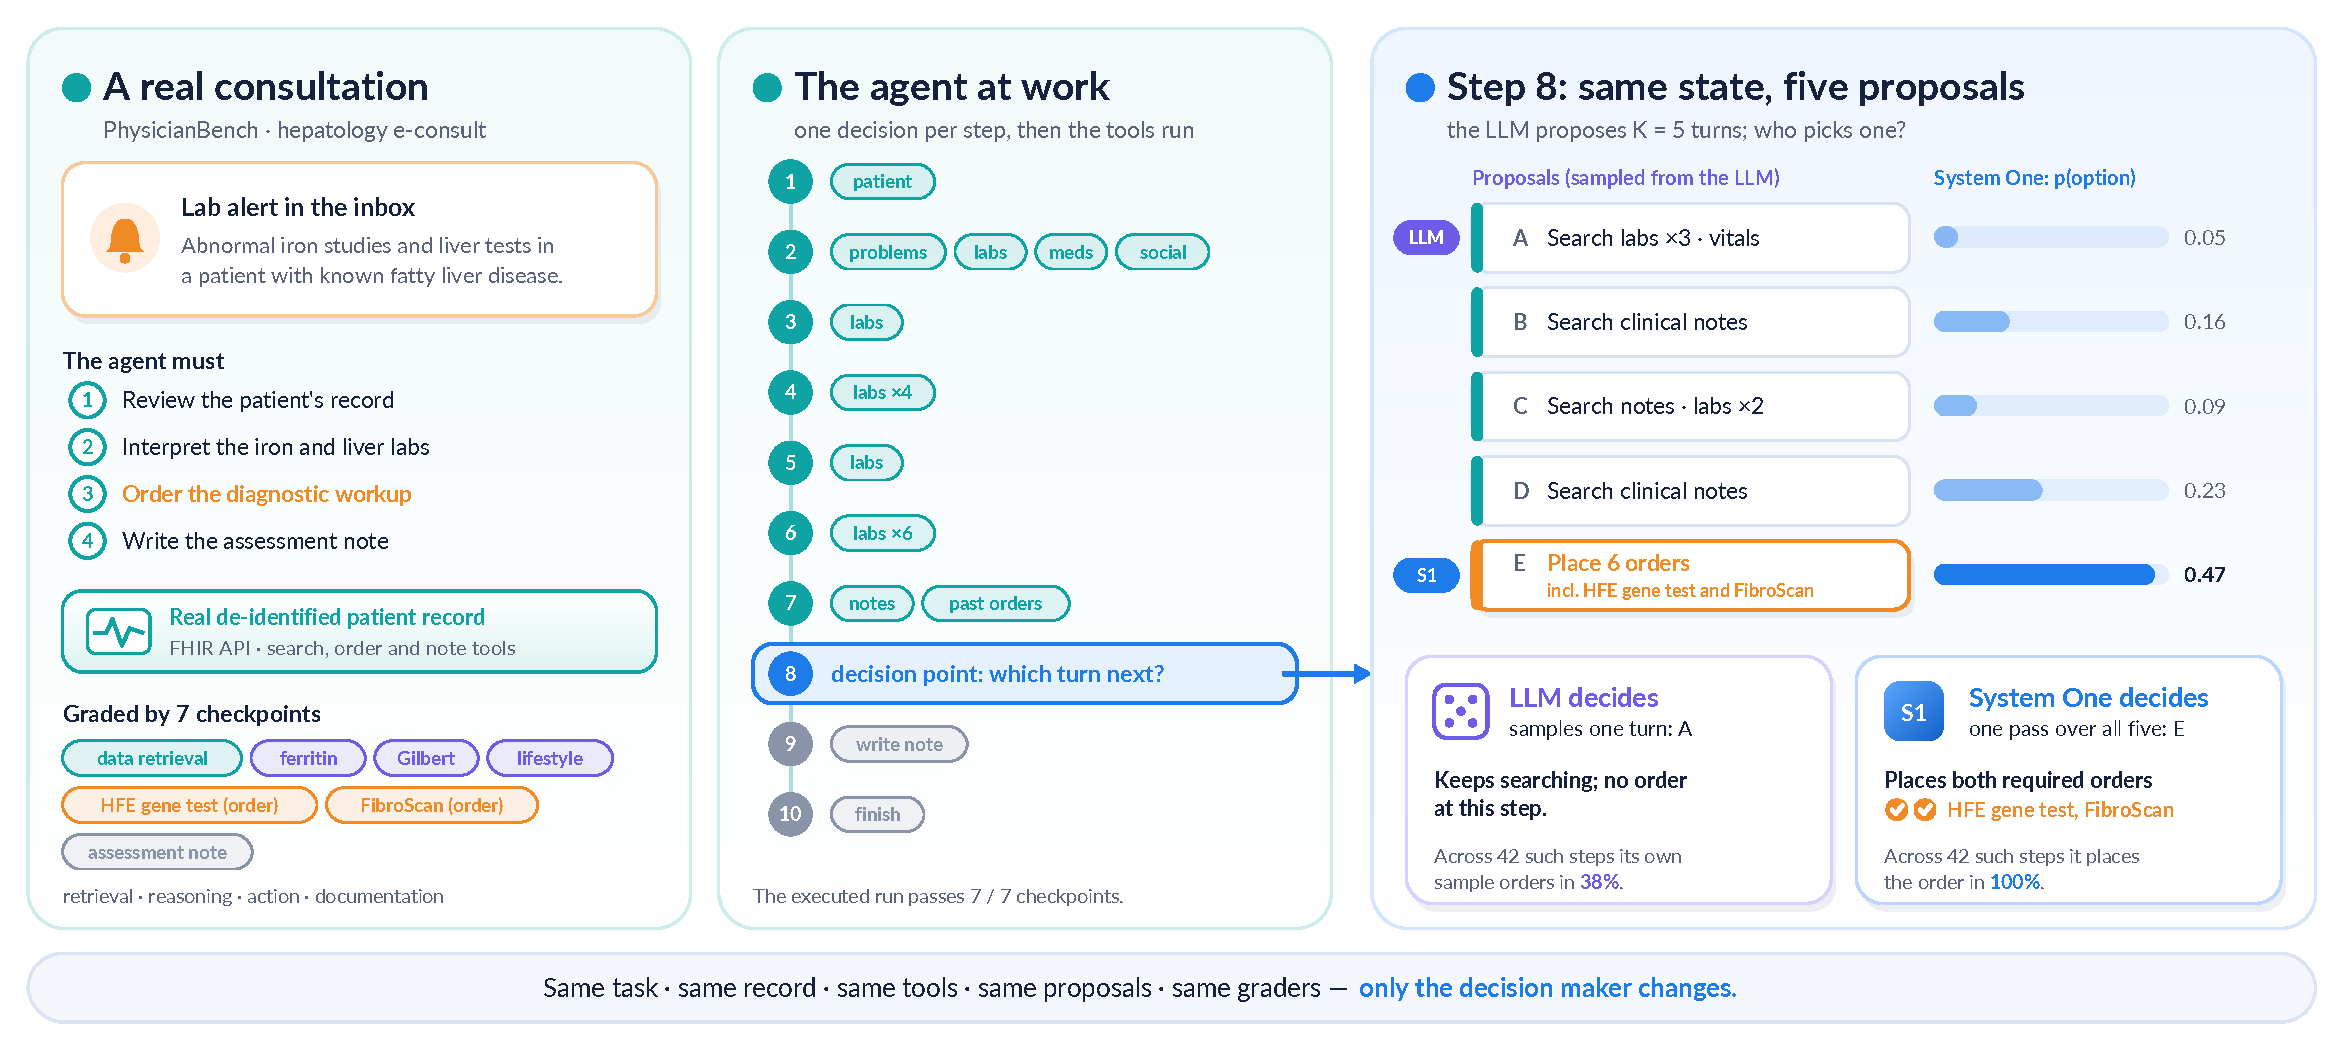
\includegraphics[width=\textwidth]{fig0_case.pdf}
\caption{\textbf{One real consultation, one decision, two deciders.} A PhysicianBench task (instruction paraphrased):
a hepatology e-consult on abnormal iron and liver tests, in which the agent must review the record, interpret the labs,
order the workup and write a note, graded by seven checkpoints. At step 8 the LLM has proposed five next turns. Its
own sample (A) keeps searching labs. The System One model reads the same state and all five proposals in one forward
pass and puts the most probability on E, which places both orders the graders require. Across all \ONReqn{} order
steps where a proposal places a required order, the LLM's own sample orders in \ONReqfirst\% and Clef in
\ONReqclef\%; most of the LLM's misses are placed at a later step (\S\ref{sec:timing}). The figure shows tool types,
probabilities and outcomes only, never patient data.}
\label{fig:case}
\end{figure*}

\begin{figure*}[t]
\centering
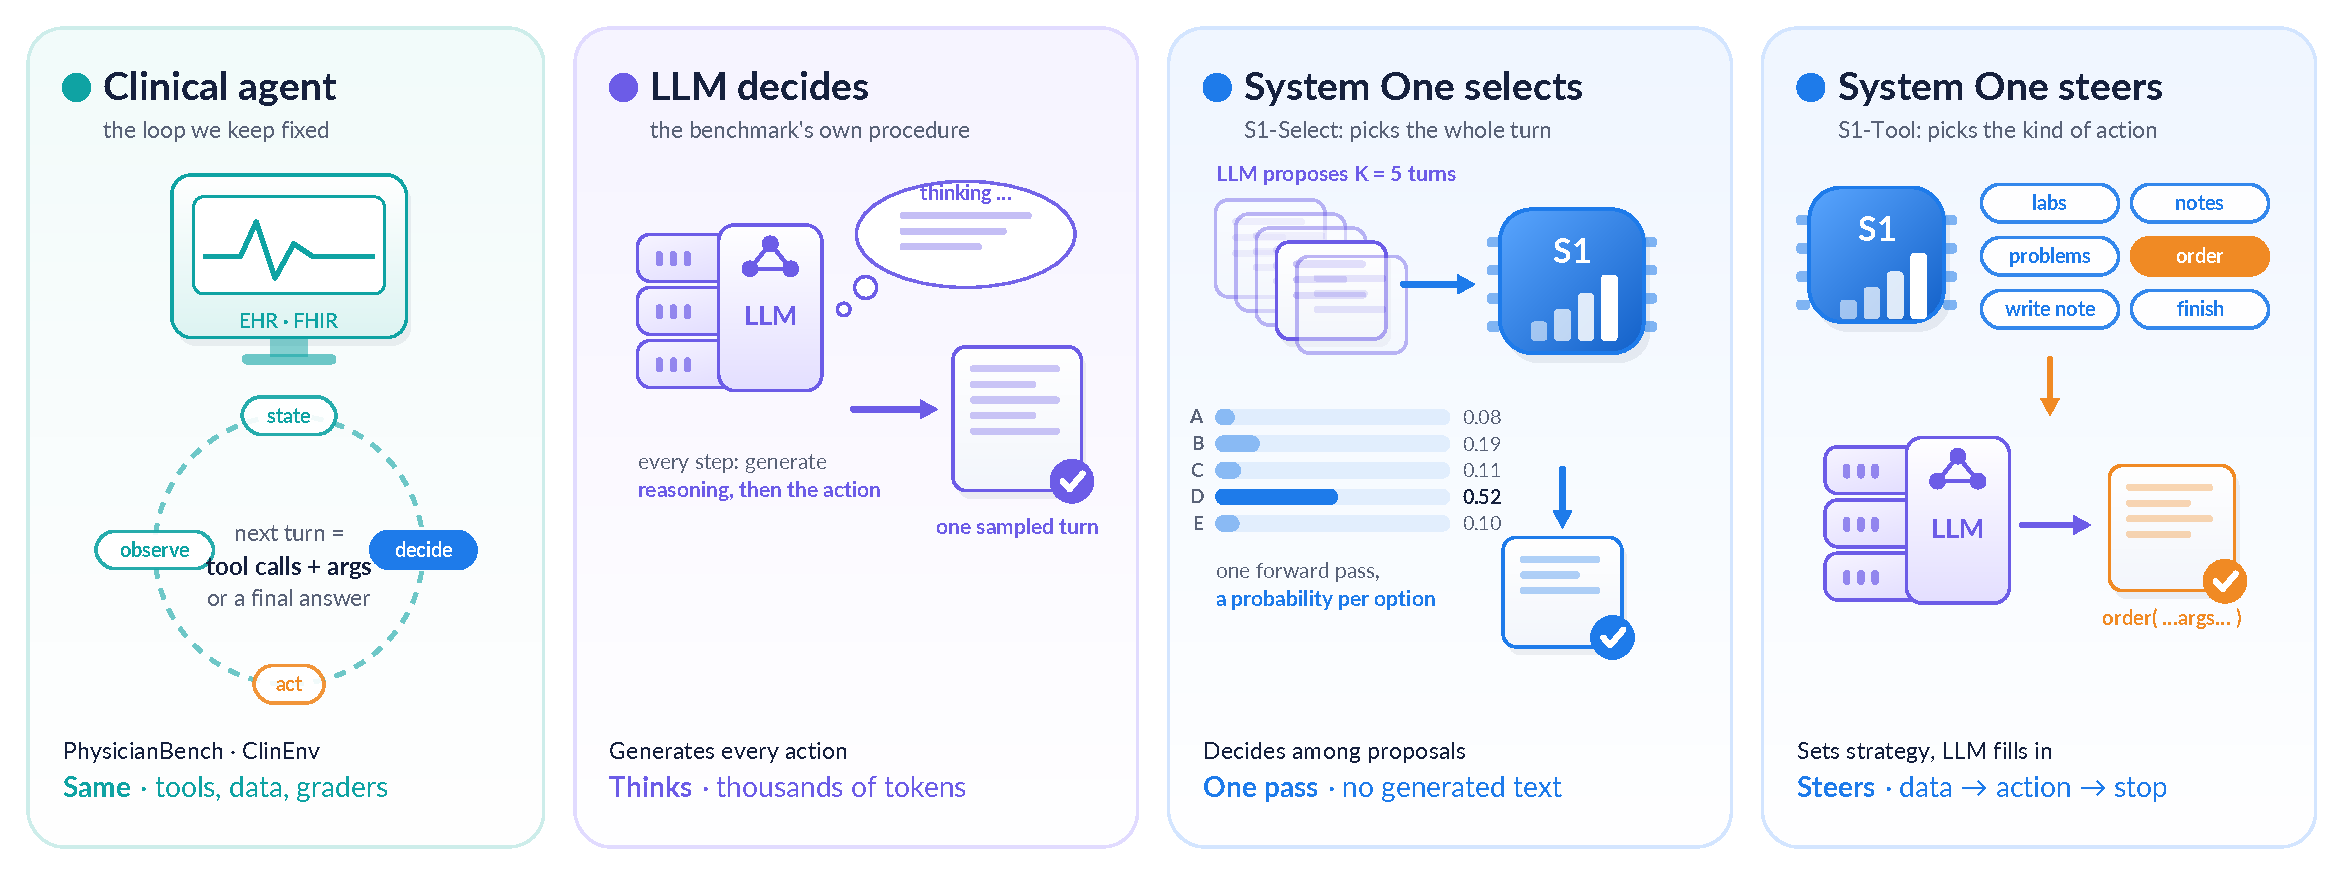
\includegraphics[width=\textwidth]{fig1_overview.pdf}
\caption{\textbf{Ways to make the next decision in the same clinical agent loop.} The loop, tools, records and
graders stay fixed. \llm: the model samples its next turn after reasoning. \sel: the LLM proposes five complete turns
and a System One model picks one in a single forward pass. \tool: the System One model picks the kind of action from
the full tool menu and the LLM writes the call. A gated variant of \sel{} (\S\ref{sec:protocol}) consults the System
One model only at order steps.}
\label{fig:overview}
\end{figure*}
\subsection{Putting a System One model in the decision seat}\label{sec:protocol}

An agent loop alternates between a state $s_t$, the task plus every action and result so far, and the next turn
$a_t$: a set of tool calls with arguments, or a final answer. The benchmark samples $a_t \sim \pi(\cdot\mid s_t)$ from
the LLM. We replace only this step.

\paragraph{\llm{} (reference).} One sample from $\pi$ with thinking on and the model's default sampling, exactly as
the benchmark prescribes. A logging variant samples $K{=}5$ turns and executes the first, which has the same
distribution as \llm{} and gives the run-to-run noise floor.

\paragraph{\sel{}: the System One model chooses the turn.} The LLM samples $K{=}5$ turns $a_t^{(1)},\dots,a_t^{(5)}$
i.i.d.\ from $\pi$ in one request. Exact duplicates are merged. The System One model reads the state and the distinct
turns, rendered as tool calls with full arguments, and returns a probability for each; the most probable turn is
executed. It never sees the LLM's reasoning, so it judges actions, not rationales. A uniform pick among $K$ i.i.d.\
samples has the same distribution as \llm, so any difference between the two comes from \emph{which} sample is chosen.

\paragraph{\tool{}: the System One model chooses the kind of action.} The System One model reads the state and the
full tool menu (each tool's name and description, plus \textsc{finish}) and picks one. The LLM then writes the turn
with its calls constrained to the chosen tool. The System One model now sets the agent's strategy and timing, and the
LLM supplies the content. \ctl{} is the control: the same one-tool-per-turn restriction with the LLM choosing (it keeps
only the calls of its own turn's first tool).

\paragraph{Gated selection: System One plus the reasoning LLM.} The System One model is consulted only at some steps
and only overrules the LLM's own first sample there. In the variant we test online it is consulted only where at
least one proposal places a service or medication order; elsewhere, including every choice between finishing,
writing the note and gathering more data, the LLM's first sample is executed. A margin variant overrules only when the
System One model prefers its pick to the LLM's sample by a log-odds margin.

\paragraph{Fair inputs.} Options are named by letters shuffled with a seed per task, run and step. The System One model
reads a deterministic 32k-token view of the state (oldest tool results shortened first); the LLM reads up to 128k
tokens. If the System One model fails, the first sample is executed; this happened \DECSelerr{} times in the
\sel{} run.
\begin{table*}[t]
\centering\small
\begin{tabular}{@{}lrrrrrrrrrr@{}}\toprule
& \multicolumn{2}{c}{Task pass@1} & \multicolumn{2}{c}{All checkpoints} & \multicolumn{4}{c}{Checkpoints by type (\%)} & & \\
\cmidrule(lr){2-3}\cmidrule(lr){4-5}\cmidrule(lr){6-9}
Decision maker & \% & $\Delta$ [95\% CI] & \% & $\Delta$ [95\% CI] & DR & CR & AE & Doc & \shortstack{Calls\\/task} & \shortstack{Tokens\\/task} \\\midrule
\textsc{LLM} & \textbf{41.0} & \textit{ref.} & \textbf{81.3} & \textit{ref.} & 83.2 & \textbf{84.1} & 75.0 & \textbf{70.7} & 36.3 & 29k \\
\textsc{S1-Select} & 37.0 & $-$4.0 [$-$13.0, +5.0] & 80.2 & $-$1.1 [$-$4.7, +2.6] & \textbf{85.0} & 82.8 & \textbf{80.1} & 65.7 & 31.2 & 119k \\
\textsc{S1-Tool} & 7.0 & $-$34.0 [$-$45.0, $-$23.0] & 44.3 & $-$37.0 [$-$44.5, $-$29.3] & 44.7 & 47.5 & 52.3 & 26.3 & 25.7 & 18k \\
\bottomrule\end{tabular}

\caption{\textbf{PhysicianBench, run 1, \PBpaired{} tasks completed by all three decision makers} (Clef as the System
One model). $\Delta$: difference from \llm{} in points with a 95\% task bootstrap interval. Checkpoint types: data
retrieval (DR), clinical reasoning (CR), action execution (AE), documentation (Doc). Calls: tool calls per task.
Tokens: generated tokens per task, including all five proposals for \sel. Bold: best per column.}
\label{tab:main}
\end{table*}

\begin{figure*}[t]
\centering
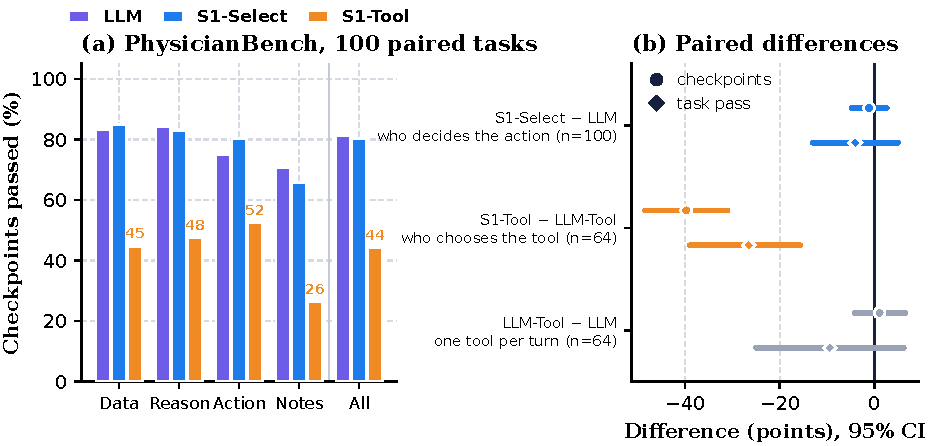
\includegraphics[width=\textwidth]{fig2_main.pdf}
\caption{\textbf{A System One model keeps the LLM's quality when it chooses among proposals, and falls behind when it
steers.} (a) Checkpoint success by type on the paired tasks. (b) Paired differences with 95\% intervals, each on the
tasks both arms completed.}
\label{fig:main}
\end{figure*}
\subsection{Performance: choosing among proposals}\label{sec:select}

Table~\ref{tab:main} and Figure~\ref{fig:main} give the headline for Clef. \sel{} passes \PBcpSel\% of checkpoints
against \PBcpLLM\% for the LLM ($\Delta$ \PBdiffSel{} points in task success, McNemar $p\PBpSel$). The noise floor is
wide: two runs of the same LLM policy differ on \PBnfDisc{} of 100 tasks ($\Delta$ \PBnfDiff{} points), so single-run
differences in task success of a few points carry no signal. Pooling the LLM's runs sharpens the checkpoint-level
comparison (Table~\ref{tab:pooled}).

\begin{table}[t]
\centering\small
\resizebox{\columnwidth}{!}{%
\begin{tabular}{@{}lccc@{}}\toprule
& \llm{} & Clef & pplx-decider \\
& (pooled) & (100 tasks) & (100 tasks) \\\midrule
Task pass & 0.41 & $-$0.04 [$-$0.12, 0.03] & +0.04 [$-$0.06, 0.14] \\
Required-order cp. & 0.76 & +0.01 [$-$0.06, 0.07] & +0.04 [$-$0.05, 0.14] \\
Documentation cp. & 0.70 & $-$0.04 [$-$0.11, 0.03] & +0.03 [$-$0.05, 0.12] \\
Required orders placed & 0.68 & $-$0.02 [$-$0.10, 0.05] & +0.05 [$-$0.05, 0.15] \\
Notes written & 1.5 & \textbf{$-$0.38} [$-$0.60, $-$0.09] & \textbf{$-$0.52} [$-$0.68, $-$0.37] \\
Retrieval before 1st action & 30 & \textbf{$-$5.5} [$-$8.0, $-$3.1] & \textbf{$-$3.2} [$-$5.6, $-$1.0] \\
Steps & 36 & \textbf{$-$5.1} [$-$8.1, $-$1.9] & \textbf{$-$4.0} [$-$6.7, $-$1.5] \\
\bottomrule\end{tabular}}
\caption{\textbf{\sel{} against the pooled LLM runs}, paired by task (differences with 95\% task bootstrap intervals;
LLM column: the level on the 100 paired tasks). cp.: checkpoint pass rate. Bold: interval excludes 0.}
\label{tab:pooled}
\end{table}

Neither System One model moves the checkpoints. An early gain of pplx-decider-v1.2 on required orders failed a
pre-registered replication (\S\ref{sec:timing}). Both shorten the episode: they act after less retrieval, write fewer notes and take
fewer steps. Documentation checkpoints dip by 2--4 points, within noise. Nothing in our data establishes a gain in
task success.

\subsection{Deciding is not the bottleneck}\label{sec:timing}

Why does a better pick not show up in the outcome? On the fixed exam every decider makes far fewer key errors than
the LLM's own sample (0.17--0.27 against 0.48; \S\ref{sec:commit}), yet online the checkpoints do not move. Following
each required order along the LLM's own trajectories resolves the gap (Table~\ref{tab:ceiling}). Of the 94 steps at
which the LLM's sample skipped an available required order, 79\% are followed by that order later in the same run:
the step-level key mostly rewards ordering early, not ordering at all. Of all 118 required orders in 54 tasks, the LLM
places 69\%, 11\% are proposed at some step but never executed, and 19\% are never proposed by any sample. Selection
can at most recover the 11\% (on these trajectories, 4 more of 54 tasks would pass); the 19\% are bounded by
generation. The decision seat holds little of the LLM's error.

pplx-decider-v1.2 shows what a selector does with that margin. It recovers part of it (proposed but never executed:
4\% against 11\%, $-$7 points [$-$13, 0]) and gives about as much back on generation: it acts after less retrieval, and
4 points more of the required orders are never proposed ([$-$5, 13]). It places about as many as the LLM (+3 [$-$8,
12]). Its apparent gain on its first 76 tasks (+13 points on required-order checkpoints) failed a pre-registered
replication on the 24 tasks it had not run ($-$18 [$-$36, $-$2], against an LLM that already passes 84\% of them).

The exam cannot see any of this. Restricted to steps where the counterfactual is known (the LLM's sample takes no open
required order and a proposal places one the run never places), it holds only 11 questions in 9 tasks, too few to
rank deciders (take rates 0.64--0.91, intervals $\pm$0.2--0.3). Step-level answer keys inside an agent's own
trajectory measure decision \emph{style}; only whole runs rank deciders on outcome. Appendix~\ref{app:frontier}
does this for 60 decisions, continuing every option to the agent's finish: no judge, System One or LLM, beats the
agent's own pick reliably.


\subsection{Mechanism: a commitment bias}\label{sec:commit}

Why do the System One models shorten the episode? The fixed exam answers
on identical inputs (Tables~\ref{tab:exam} and \ref{tab:errors}). All six models agree with the LLM's own sample
about as often as a random pick would (21--27\% for five of them, 36\% for linne-oak-1.0; random \EXagreeRandom\%), and with each other
more often. They make far fewer key errors than the LLM's sample (0.17--0.27 against 0.48; every bootstrap interval
excludes 0), but the errors move rather than vanish: the LLM omits an available required order at 55\% of such steps
and the deciders at 2--18\%, while the deciders order when no required order is on offer at 52--71\% of steps against
the LLM's 35\%, and finish while a required order is open at 90--97\% of such steps against 80\%.

\begin{table}[t]
\centering\small
\resizebox{\columnwidth}{!}{%
\begin{tabular}{@{}lrrrrr@{}}\toprule
& Error & Omits & Over- & Finishes & Redun- \\
& (3 keys) & required & orders & early & dant \\\midrule
\llm{} (own sample) & 0.48 & 55 & 35 & 80 & 28 \\
Always order (no model) & 0.22 & 0 & 100 & 77 & 25 \\\midrule
Clef-27B & 0.19 & 2 & 66 & 90 & 8 \\
pplx-decider-v1.2 & \textbf{0.17} & 3 & 71 & 90 & 4 \\
d3 & 0.18 & 4 & 67 & 90 & 4 \\
linne-oak-1.0 & 0.21 & 5 & 53 & 97 & 9 \\
amos-1-large & 0.27 & 18 & 53 & 90 & 11 \\
decider-31b & 0.21 & 7 & 52 & 93 & 8 \\\bottomrule
\end{tabular}}
\caption{\textbf{Error profile on the fixed exam} (1,460 questions answered by all six, 100 tasks; 200 keyed: 97
order, 30 finish, 85 redundancy). Error: bad picks over all (question, key) pairs. Other columns in \%: omits a
required order on offer; orders when none is required among mixed options; finishes while a required order is open;
picks a redundant option. Always order: take the most-sampled ordering option whenever one is offered.}
\label{tab:errors}
\end{table}

Two observations show that much of this is a preference over kinds of action rather than a reading of the patient.
First, a rule with no model, \emph{always take an ordering turn when one is offered}, reaches an error of 0.22 and
leaves no required order behind; on the order key it is better than every decider. Second, the deciders' low
redundancy is not evidence that they track what has been done: in 17--18 of the 19--22 questions where a decider
avoids the LLM's redundant option, it does so by choosing \textsc{finish} over a rewrite of the note. Table~\ref{tab:commit}
puts the preference in one number per kind: every model picks ordering turns 1.3--1.6$\times$ and finishing turns
1.3--1.4$\times$ as often as the LLM's own sample does, and retrieval turns 0.89--0.93$\times$. The same profile shows
online (Table~\ref{tab:pooled}: less retrieval before acting, fewer notes, shorter runs). We call it a
\emph{commitment bias}: System One deciders prefer turns that commit (order, write, finish) over turns that gather
information.

\begin{table}[t]
\centering\small
\begin{tabular}{@{}lrrrr@{}}\toprule
& Order & Finish & Note & Retrieve \\\midrule
Clef-27B & 1.57 & 1.34 & 1.06 & 0.89 \\
pplx-decider-v1.2 & 1.49 & 1.35 & 1.09 & 0.90 \\
d3 & 1.48 & 1.37 & 1.09 & 0.90 \\
linne-oak-1.0 & 1.37 & 1.43 & 1.18 & 0.89 \\
amos-1-large & 1.29 & 1.30 & 1.06 & 0.93 \\
decider-31b & 1.36 & 1.41 & 1.18 & 0.89 \\\bottomrule
\end{tabular}
\caption{\textbf{The commitment bias.} Picks of each kind of turn on the exam, relative to the LLM's own sample on the
same questions ($>1$: chosen more often than the LLM chooses it).}
\label{tab:commit}
\end{table}

The bias is useful exactly where the LLM under-commits, and it costs elsewhere. pplx-decider-v1.2 online takes more
of the required orders that a proposal offers (offered but never executed: 4\% of required orders, against 11\% for
the LLM; difference $-$7 points [$-$13, 0]), but 4 points more are never proposed at all ([$-$5, 13]), so it places
about as many as the LLM (+3 [$-$8, 12]). Clef does not even gain the first part: on its own trajectories it places 6 points fewer of the required orders than
the LLM ([$-$15, 3]), and 8 points more of them are never proposed at all ([$-$1, 18]), plausibly because it moves to
action after less retrieval and the LLM then never thinks of them.

\paragraph{A prior and a misreading (blind test, pre-registered).} Does the bias read the patient at all? We asked
pplx-decider-v1.2 the whole exam again with the options but no state (same option letters; test P4, fixed before its
data existed). The pre-registered style hypothesis, that blind and informed picks agree on at least 60\% of questions
and the order and finish errors move by at most 0.05, is rejected: they agree on 41\% (random 22\%), and blind picks
match the kind of the informed pick barely more often than chance (91\% against 88\%; other deciders with the state:
95--98\%). The model reads the state. But the keys move in opposite directions (Table~\ref{tab:blind}). On orders,
the blind model is already far better than chance: about two thirds of the reduction from a random pick needs no
patient state, so the order preference is largely a prior over what the options look like. On redundancy, the state
does most of the work. On finishing, the state hurts: these are late steps where 73\% of the options are
\textsc{finish} and the LLM itself mostly wants to stop. Blind, the decider avoids finishing (below chance); with the
state, it finishes while a required order is open more often than chance and more often than the LLM's own sample.
The premature finishing is thus a misreading of the state, which agrees with, and strengthens, the LLM's own sense
that the case is done.

\begin{table}[t]
\centering\small
\resizebox{\columnwidth}{!}{%
\begin{tabular}{@{}lrrrr@{}}\toprule
Key error & Random & Blind & State & Blind $-$ state \\\midrule
Order (97 q.) & 0.55 & 0.22 & 0.07 & $+$0.14 [0.08, 0.21] \\
Redundancy (86) & 0.35 & 0.24 & 0.03 & $+$0.21 [0.11, 0.31] \\
Finish (30) & 0.73 & 0.53 & 0.90 & $-$0.37 [$-$0.53, $-$0.19] \\\bottomrule
\end{tabular}}
\caption{\textbf{Blind test (P4), pplx-decider-v1.2.} Key errors of a random option, of the decider without the patient
state (options only) and with it; differences with task-bootstrap 95\% CIs. The LLM's own sample: 0.55, 0.28, 0.80.}
\label{tab:blind}
\end{table}

\subsection{Steering alone, the bias breaks the agent}\label{sec:steer}

Given the tool menu instead of proposals, the same model fails. \tool{} passes \PBpassTool\% of tasks and
\PBcpTool\% of checkpoints ($\Delta$ \PBdiffTool{} points in task success, $p\PBpTool$). It retrieves \TLRetTool{}
times per task against the LLM's \TLRetLLM{}, starts acting after \TLFirstTool{} retrieval calls instead of
\TLFirstLLM, and writes the note \TLDocTool{} times, rewriting it again and again; it chooses to write the note at
\TCwriteClef\% of steps, where the LLM does so at \TCwriteLLM\% (Table~\ref{tab:toolchoice}). Restricting the LLM to
one tool per turn costs nothing measurable (\ctl{} versus \llm: \PRCtlLLMcp{} checkpoint points), while handing the
same restricted choice to the System One model costs \PRToolCtlcp{} points. pplx-decider-v1.2 in the same seat falls
behind as well (\ONToolPplxcp{} points over \ONToolPplxn{} tasks). In an open action space the commitment bias has
nothing to anchor it: committing means writing, and the agent writes instead of looking.

\begin{table}[t]
\centering\small
\begin{tabular}{@{}lrr@{}}\toprule
Tool & \shortstack{Clef\\(\tool)} & \shortstack{LLM\\(\ctl)} \\\midrule
Write note & 44 & 8 \\
Search labs & 18 & 29 \\
Search notes & 10 & 20 \\
Search problems & 4 & 9 \\
Demographics & 5 & 5 \\
Search med.\ orders & 3 & 6 \\
Place order & 6 & 3 \\
Finish & 4 & 4 \\
\bottomrule\end{tabular}

\caption{\textbf{Which tool each decider picks} under the same one-tool-per-turn restriction, as a share of steps
(\%), on the tasks both completed.}
\label{tab:toolchoice}
\end{table}

\begin{figure}[t]
\centering
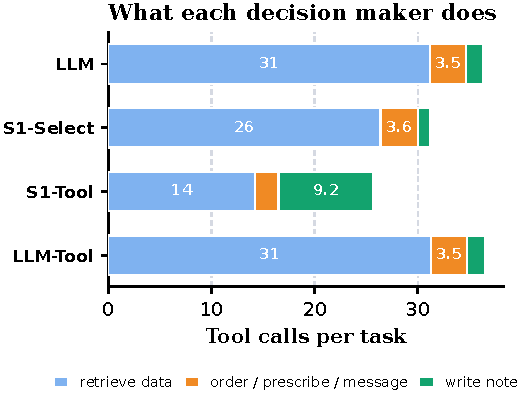
\includegraphics[width=\columnwidth]{fig4_tools.pdf}
\caption{\textbf{Tool calls per task by kind.} Steering, the System One model under-retrieves and over-documents.
\ctl{}: the LLM under the same one-tool-per-turn restriction, on the tasks it shares with \tool.}
\label{fig:tools}
\end{figure}

\subsection{Boundaries: where a System One decider is reliable}\label{sec:boundaries}

On the keyed exam questions we split the benefit of executing the decider's pick instead of the LLM's sample (key
errors avoided per question) by what the decider and the LLM signal (Clef and pplx-decider-v1.2 shown; the other models behave alike).

\paragraph{Its confidence is informative.} Overrides where the decider prefers its pick to the LLM's sample by a
log-odds of at least 3 avoid 0.8--1.0 order-key errors per question and 0.6 redundancy errors; overrides below 1.5
avoid almost none. A margin keeps most of the benefit with far fewer overrides.

\paragraph{It helps where the reasoning model is unsure.} When only 1--2 of the LLM's five samples are semantically
the same decision as its first sample (same tools and key clinical arguments), the decider avoids 0.37--0.40 errors
per question; at 4 of 5 it avoids 0.11--0.17, and at 5 of 5 none. Order decisions sit almost entirely at 1 of 5. The
LLM's self-consistency and the decider's confidence are complementary signals for when to hand over.

\paragraph{Finishing is its blind spot.} Where the decider confidently overrules the LLM's sample toward
\textsc{finish} while a required order is still open, it is wrong in 4 of 5 cases (error change $-$0.75 to $-$0.80,
$n=4$--5), and every model finishes early more often than the LLM (Table~\ref{tab:errors}). In \tool{} the same
blindness appears as an agent that never stops writing.

\paragraph{Long states.} 85\% of keyed questions exceed the decider's 32k window and are read with shortened tool
results. The deciders' error is 0.03--0.07 on the questions read in full and 0.20--0.23 on shortened ones, against
0.44--0.47 and 0.51--0.52 for the LLM's sample; long, truncated trajectories are where the System One view is weakest
(confounded with late steps).

\subsection{Other System One models in the same seat}\label{sec:deciders}

Is this Clef's behaviour, or how System One models behave as deciders? We put five other open System One models in
the same seat: pplx-decider-v1.2, d3, linne-oak-1.0, amos-1-large and decider-31b. Each runs its authors' own
serving code at a pinned revision, and nothing else changes: the same rendering, question wording and 32k fitting
rule (Appendix~\ref{app:interface}).

\paragraph{The same exam for every decider.} The LLM runs every task once and logs, at each step, its five
candidate turns and the full state. Each step with at least two distinct candidates becomes a question, so far
\EXquestions{} questions from \EXtasks{} tasks. Every decider answers byte-identical requests: the same state, the
same options and the same option letters. The comparison is restricted to the \EXcommon{} questions that all of
them have answered. On order steps the task graders give an answer key (\EXkeyed{} questions that separate right
from other options). Table~\ref{tab:exam} reports the result. On order steps, all three
deciders pick a right option far more often than the LLM's own sample (Clef \EXaccClef\%, pplx-decider-v1.2
\EXaccPplx\%, d3 \EXaccDthree\%, against \EXaccFirst\% for the LLM and \EXaccRandom\% at random). When a proposal
places a required order, every one of them takes it (\EXreqClef\%, \EXreqPplx\% and \EXreqDthree\%; the LLM
\EXreqFirst\%). The bias toward action is shared too: when no proposal places a required order, they still order
in \EXnoneClef\%, \EXnonePplx\% and \EXnoneDthree\% of steps, the LLM in \EXnoneFirst\%. Across all questions
they agree with the LLM's own sample about as often as a random pick would (\EXagreeClef\%, \EXagreePplx\% and
\EXagreeDthree\%; random \EXagreeRandom\%), and with each other more often (pplx-decider-v1.2 and d3 on
\EXpairPplxDthree\% of questions). Taking the required action is how System One deciders behave, not a quirk of
Clef.

\paragraph{Whole tasks.} We also rerun the online arms with pplx-decider-v1.2 in Clef's seat
(Table~\ref{tab:deciders}). Choosing among proposals, it again stays level with the LLM
(\ONSelPplxcp{} checkpoint points over \ONSelPplxn{} tasks). Steering, it again falls far behind the same
restriction with the LLM choosing (\ONToolPplxcp{} points over \ONToolPplxn{} tasks). Both online findings hold for a second System One model.

\begin{table}[t]
\centering\small
\resizebox{\columnwidth}{!}{\begin{tabular}{@{}lrrrrrr@{}}\toprule
& \multicolumn{3}{c}{Order steps (answer key)} & \multicolumn{3}{c}{All questions} \\
\cmidrule(lr){2-4}\cmidrule(l){5-7}
Decider & Right & \shortstack{Orders,\\required} & \shortstack{Orders,\\none req.} & \shortstack{Agrees\\w/ LLM} & Act & Note \\
\midrule
Random & 45 & -- & -- & 22 & -- & -- \\
\llm{} (own sample) & 45 & 45 & 35 & 100 & -- & -- \\
\llm{} (most sampled) & 45 & -- & -- & -- & -- & -- \\
\midrule
Clef-27B & 94 & 98 & 66 & 23 & 15 & 10 \\
pplx-decider-v1.2 & 93 & 97 & 71 & 27 & 14 & 11 \\
d3 & 91 & 96 & 67 & 21 & 14 & 11 \\
linne-oak-1.0 & 92 & 95 & 53 & 37 & 13 & 11 \\
amos-1-large & 78 & 82 & 53 & 22 & 12 & 10 \\
decider-31b & 91 & 93 & 52 & 24 & 13 & 11 \\
\bottomrule\end{tabular}
}
\caption{\textbf{The same exam for every decider} (PhysicianBench, the LLM's own logged states and candidates;
\EXcommon{} questions answered by every decider, \EXkeyed{} of them with an answer key). Right: picks a required
order on order steps where options differ. Orders, required / none req.: picks an ordering option when one places a
required order, or when none does. Agrees w/ LLM: same pick as the LLM's own sample. Act, Note: share of all picks
that place orders or write the note. Preliminary: the exam and the remaining deciders are still running.}
\label{tab:exam}
\end{table}

\begin{table}[t]
\centering\small
\resizebox{\columnwidth}{!}{\begin{tabular}{@{}lrrrr@{}}\toprule
& \multicolumn{2}{c}{\sel{} vs \llm} & \multicolumn{2}{c}{\tool{} vs \textsc{LLM-Tool}} \\
\cmidrule(lr){2-3}\cmidrule(l){4-5}
Decider & Tasks & $\Delta$ checkpoints & Tasks & $\Delta$ checkpoints \\
\midrule
Clef-27B & 100 & $-$1.1 [$-$4.7, +2.7] & 94 & $-$38.1 [$-$45.2, $-$31.1] \\
pplx-decider-v1.2 & 76 & +1.1 [$-$4.9, +7.1] & 49 & $-$24.7 [$-$35.0, $-$14.8] \\
\bottomrule\end{tabular}
}
\caption{\textbf{Whole tasks with another decider in Clef's seat.} Paired checkpoint differences with 95\% intervals,
each on the tasks both arms have completed.}
\label{tab:deciders}
\end{table}


\subsection{System One plus the reasoning LLM}\label{sec:gate}

The boundaries suggest a narrower role. Let the LLM gather data, write the note and decide when to stop; consult the
System One model only where a proposal places an order, the decisions it gets right and the LLM defers. On the exam,
this \emph{orders-only} gate keeps the decider's order behaviour (pplx-decider-v1.2: omission 3\%) and leaves finishing
and redundancy at the LLM's level, while overruling the LLM on 11\% of steps instead of 73\%. Gating at every order or
finish step overrules on 19\%; a gate by log-odds margin or by the LLM's self-consistency does not lower the exam
error further under cross-validation, because the exam's redundancy key rewards finishing over a note rewrite and the
keys pull against each other. The exam cannot choose among these designs; whole runs must.

\paragraph{Pre-registered online tests.} We fixed these tests before their data existed.
\textbf{P1} replicated pplx-decider-v1.2 in \sel{} on the 24 tasks it had not run; prediction: more required-order
checkpoints than the pooled LLM runs. It failed ($-$18 points [$-$36, $-$2], 16 tasks with such checkpoints;
\S\ref{sec:select}).
\textbf{P2$'$} ran the orders-only gate with pplx-decider-v1.2 on all 100 tasks; prediction: the required-order gain
of \sel{} (which P1 has since failed to replicate) without its loss of notes (notes within the LLM's run-to-run noise);
documentation not lower; task pass claimed only if its CI excludes 0. The primary prediction fails: required-order
checkpoints $+$5 points [$-$2, 14]. Table~\ref{tab:gate} pools this run with a second one (P5, below). The secondary ones hold: notes and steps
return to the LLM's level, and documentation is not significantly lower. Task pass does not change. The design does
what the blind test (P4, \S\ref{sec:commit}) predicts for its structure: away from finishing, the decider no longer
stops the agent early. What it cannot do is pass the ceiling of \S\ref{sec:timing}.

\begin{table*}[t]
\centering\small
\caption{Online, all 100 tasks: the orders-only gate (two runs, pooled) and full steering in \sel{} (one run), both with
pplx-decider-v1.2, each minus the pooled LLM runs, with task-bootstrap 95\% CIs; the last column is the difference between two LLM runs
(run-to-run noise). Required orders: the 54 tasks with such checkpoints.}\label{tab:gate}
\begin{tabular}{lccc}
\toprule
& gate $-$ LLM & \sel{} $-$ LLM & LLM $-$ LLM \\
\midrule
required-order checkpoints & $+$0.06 [$-$0.01, 0.14] & $+$0.04 [$-$0.05, 0.14] & -- \\
required orders placed & $+$0.04 [$-$0.03, 0.12] & $+$0.05 [$-$0.05, 0.15] & $+$0.05 [$-$0.01, 0.11] \\
orders placed per task & $\mathbf{+0.95}$ [0.51, 1.44] & $+$0.26 [$-$0.35, 0.93] & $+$0.18 [$-$0.34, 0.71] \\
\quad of which not in the rubric & $\mathbf{+0.74}$ [0.20, 1.31] & $+$0.21 [$-$0.70, 1.11] & $+$0.35 [$-$0.31, 1.02] \\
notes written per task & $-$0.07 [$-$0.26, 0.12] & $\mathbf{-0.52}$ [$-$0.68, $-$0.37] & $-$0.12 [$-$0.40, 0.15] \\
steps per task & $-$0.5 [$-$3.9, 3.2] & $\mathbf{-4.0}$ [$-$6.7, $-$1.5] & -- \\
Documentation checkpoints & $-$0.03 [$-$0.09, 0.04] & $+$0.03 [$-$0.05, 0.12] & -- \\
task pass & $-$0.01 [$-$0.09, 0.06] & $+$0.04 [$-$0.06, 0.14] & -- \\
\bottomrule
\end{tabular}
\end{table*}

\paragraph{The gate over-orders.} In the P2$'$ run the gated agent placed 1.3 more orders per task than the LLM
[0.76, 1.89], nearly all matching no order in the rubric [$+$1.13, 0.52 to 1.79]. We saw this after the fact and
pre-registered a replication, \textbf{P5}: a second gate run, predicting more orders (at least $+$0.5, CI excluding 0)
and more orders outside the rubric (CI excluding 0). The first half replicates ($+$0.61 [0.12, 1.13]); the second
does not reach significance in the second run alone ($+$0.35 [$-$0.29, 0.97]). Pooled over both runs
(Table~\ref{tab:gate}) the gate places 0.95 more orders per task, 0.74 of them outside the rubric. Full steering does not show this, plausibly because it ends runs
earlier and so gives the order prior fewer steps to act on; the gated agent runs as long as the LLM, and at every
order step the decider prefers the ordering turn. This is the state-free part of the commitment bias, now visible as
volume. PhysicianBench barely penalises it (one task forbids an order), but in practice extra orders cost money and
can harm patients.
An exploratory gate that also consults the decider at finish steps (margin 1.5, 22 tasks; not part of any test)
brings the losses back: notes $-$0.62 [$-$1.02, $-$0.29], steps $-$6.7 [$-$12.9, $-$1.9]. The harm of steering
sits at the finish step, as the blind test predicts.
\FloatBarrier
\section{Additional results on the decision seat}\label{app:results}

\begin{table*}[t]
\centering\small
\resizebox{\textwidth}{!}{\begin{tabular}{lrrrrrrrrr}
\toprule
Comparison & Tasks & Pass@1 & $\Delta$ pass@1 [95\% CI] & $p$ & $\Delta$ checkpoints [95\% CI] & $\Delta$ DR & $\Delta$ CR & $\Delta$ AE & $\Delta$ Doc \\
\midrule
\sel{} vs \llm & 100 & 37.0 / 41.0 & $-$4.0 [$-$13.0, +5.0] & 0.52 & $-$1.1 [$-$4.8, +2.7] & +1.8 & $-$1.2 & +5.1 & $-$5.1 \\
\tool{} vs \textsc{LLM-Tool} & 79 & 7.6 / 32.9 & $-$25.3 [$-$36.7, $-$15.2] & $<$0.001 & $-$37.3 [$-$44.9, $-$29.5] & $-$40.9 & $-$39.0 & $-$25.9 & $-$37.2 \\
\textsc{LLM-Tool} vs \llm & 79 & 32.9 / 40.5 & $-$7.6 [$-$20.2, +5.1] & 0.34 & +1.1 [$-$3.4, +5.8] & $-$0.2 & +2.0 & +11.4 & $-$6.4 \\
\bottomrule
\end{tabular}
}
\caption{Paired comparisons, each on the tasks both arms completed (run 1). $\Delta$ in points; per-type columns give
the point difference in checkpoint success.}
\label{tab:pairs}
\end{table*}

\begin{table*}[t]
\centering\small
\begin{tabular}{@{}lrrrrrrr@{}}\toprule
& \shortstack{Steps\\/task} & \shortstack{Distinct\\strings (\%)} & \shortstack{Distinct\\actions (\%)} & \shortstack{Mean\\max $p$} & \shortstack{Norm.\\entropy} & \shortstack{Departs from\\LLM sample (\%)} & \shortstack{Decide\\(s)} \\\midrule
\textsc{S1-Select} & 11.8 & 99 & 89 & 0.382 & 0.886 & 79 & 4.7 \\
\bottomrule\end{tabular}

\caption{\sel{} decisions, run 1. Distinct strings: steps whose five proposals are not all identical. Distinct
actions: after merging proposals with the same tools and key clinical arguments. Mean max $p$ and entropy (normalised
by $\log n$) describe the System One model's distribution where there was a choice. Departs: share of those steps where
it chose a proposal other than the LLM's first sample.}
\label{tab:decisions}
\end{table*}

\begin{figure}[t]
\centering
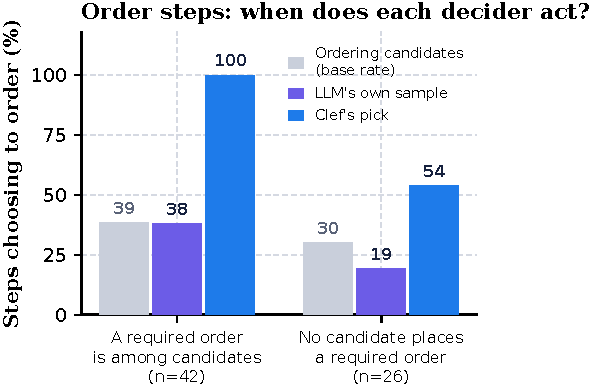
\includegraphics[width=\columnwidth]{fig3_orders.pdf}
\caption{\textbf{Clef places required orders when they are on the table.} Order steps of the \sel{} run whose
proposals mix ordering and other turns. Orders the graders do not require are not wrong, only uncredited; most of the
LLM's skipped orders are placed at a later step (\S\ref{sec:timing}).}
\label{fig:orders}
\end{figure}

Table~\ref{tab:pairs} lists every paired comparison with intervals; Table~\ref{tab:decisions} describes the decisions.
Episodes that ended without a final answer (step limit, repeated-call abort or context overflow) number \ENDLLM{} for
\llm, \ENDSel{} for \sel{} and \ENDTool{} for \tool{} on the paired tasks. Distinct proposals are semantically
different decisions at \DECSelsem\% of \sel{} steps; on the exam, 952 of 1,460 questions are choices among retrieval
turns only, which no key scores.

\end{document}
